
\documentclass{article} % For LaTeX2e
\usepackage[submission]{colm2026_conference}

\usepackage{microtype}
\usepackage{hyperref}
\usepackage{url}
\usepackage{booktabs}
\usepackage{amsmath}
\usepackage{amssymb}
\usepackage{graphicx}
\usepackage{float}
\usepackage{multirow}
\usepackage{csquotes}
\usepackage[capitalize]{cleveref}

\usepackage{lineno}

\definecolor{darkblue}{rgb}{0, 0, 0.5}
\hypersetup{colorlinks=true, citecolor=darkblue, linkcolor=darkblue, urlcolor=darkblue}


\title{Disk-onnected: Transformers Struggle to Use Their World Models}

% Authors must not appear in the submitted version.
\author{Anonymous}

\newcommand{\fix}{\marginpar{FIX}}
\newcommand{\new}{\marginpar{NEW}}

\begin{document}

\ifcolmsubmission
\linenumbers
\fi

\maketitle

\begin{abstract}
Large reasoning models collapse on Tower of Hanoi planning once the puzzle grows past a handful of disks, a failure documented behaviourally but never explained mechanistically. We ask where in the computation the failure lives: does the model never form a representation of the puzzle state, lose it across a long reasoning trace, or hold it intact and fail to act on it? We answer with two complementary studies on the flat-to-flat Tower of Hanoi. First, a small Transformer trained from scratch on solution traces is shown, through linear distance-matching probes and activation patching, to develop a linearly decodable, geometrically faithful representation of the disk configuration that reproduces the Sierpi\'nski geometry of the state graph and is causally read when the model emits a solution. Second, the same probes are applied to two frontier reasoning models, Qwen3.6-27B and DeepSeek-R1-Distill-Qwen-32B, that solve the task through extended chain-of-thought. Both encode the configuration near-perfectly at the end of the prompt, yet solve only about half of instances optimally; tracking the probe through generation reveals that the representation degrades as the model reasons, decaying from a unified planning geometry into a fragmented one at the point of commitment. Restoring the clean prompt-time representation, by injecting it at inference or by training it back into the weights with a state-encoding auxiliary loss, increases optimal-solve accuracy for Qwen3.6-27B, though the same intervention fails to transfer to DeepSeek-R1-Distill. The results reframe the reported collapse: these models build a world model and then lose it. The failure is one of maintenance, not absence, and it is at least partially recoverable.
\end{abstract}

%==============================================================================
\section{Introduction}
\label{sec:introduction}

Current models capable of drafting proofs, writing working code, and scoring at the frontier of graduate examinations cannot reliably solve a puzzle designed for children. Solving the Tower of Hanoi requires large reasoning models (LRMs) to move a stack of disks between three pegs, yet they are incapable of doing so: their accuracy falls off a cliff once the puzzle grows past a handful of disks, and, stranger still, their reasoning traces get shorter at exactly the point where the problem gets harder~\citep{shojaee2025illusion}. The behaviour has been measured carefully and named the \enquote{illusion of thinking}, but this phenomenon has not been explained mechanistically. We know that these models fail. But, we do not know what inside the model is failing.

This gap motivates a debate about what these systems are and wherein their capabilities truly lie. When a sequence model trained only to predict the next token solves a planning problem, is it manipulating an internal model of the world according to the problem it is solving, or is it recombining surface statistics with no underlying state to speak of~\citep{bender2021dangers}? The evidence so far is split. Small Transformers trained on Othello and chess move histories do build decodable causally active board representations~\citep{li2022emergent, toshniwal2022chess}; maze-solving networks encode walls and paths~\citep{spies2025transformers}. But these demonstrations so far study a model that emits one move per forward pass. None study a reasoning model that discusses, justifies and contradicts its way to an answer through thousands of tokens of chain-of-thought. This is precisely the setting in which such failures occur. The two literatures, the one documenting collapse and the other documenting world models, have never been combined into a single coherent study.

Throughout this work, we consider planning failures to be a genuine mechanistic claim, asking where they lie. For a model that collapses on a planning problem, there are three competing explanations that call for opposite solutions. (1) The model may never form a representation of the puzzle state, in which case the apparent reasoning is a facade. (2) It may form the representation but lose it somewhere across a long reasoning trace, in which case the failure is one of maintenance and the fix is a richer training signal over states. (3) Or it may hold the state intact and simply fail to act on it, in which case the failure is one of decoding and the fix lies in how the model generates. Behavioural benchmarks cannot tell these apart. Only analyzing model internals can.

We pry them apart with two different designs. First, a small Transformer trained from scratch on Tower of Hanoi solutions gives a fully controlled setting in which the existence, geometry, format, and causal role of any internal state representation can be established with probing, sparse autoencoders, and activation patching. Second, two frontier reasoning models, Qwen3.6-27B and DeepSeek-R1-Distill-Qwen-32B, are put through the same lens to test whether those findings survive at scale and under chain-of-thought. We can watch the representation evolve token by token as the model generates.


The answer that emerges is sharper than whether the model can or cannot reason. A geometrically structured world model does emerge  in models separated by orders of magnitude in size. We find that it is initially decodable, then degrades as the model reasons, from a unified planning geometry into a fragmented one at the moment the model commits to its moves. Furthermore, in one frontier model, deliberately restoring that representation, either by injecting it at inference or by training it back into the weights, recovers the lost accuracy. The illusion of thinking, it turns out, is not that the model never thinks; it is that the model forgets what it knew.


We test three hypotheses, the first two on a toy Transformer trained from scratch and the third on frontier reasoning models. \textbf{H1:} a simple autoregressive Transformer trained on flat-to-flat Tower of Hanoi traces develops a linearly decodable representation of the disk configuration. \textbf{H2:} this representation is causally implicated in the model's solution. \textbf{H3:} in large reasoning models the representation degrades over autoregressive generation, and this degradation, rather than its absence, is what drives failure.

%==============================================================================
\section{Related work}
\label{sec:related-work}

\paragraph{Planning and its failure in reasoning models.}
Reasoning models exhibit a counterintuive failure mode on long-horizon planning problems. Their accuracy collapses to zero once compositional depth exceeds a model-specific threshold, while their reasoning traces grow shorter rather than longer at the point of failure~\citep{shojaee2025illusion}. Behavioural evidence of this collapse is now well documented, but its mechanistic origin remains unclear. A separate line of work has shown that Transformer sequence models can develop internal representations of the latent state they predict over, even when trained only on next-token prediction~\citep{li2022emergent, toshniwal2022chess}. World-model emergence has been demonstrated almost exclusively in small Transformers trained on games~\citep{li2022emergent, toshniwal2022chess} or path prediction in mazes~\citep{spies2025transformers}. Whether such world models extend to large reasoning models producing extended reasoning traces is still yet to be discovered. There is a paucity in research on the question of whether a reasoning model's internal representation of a planning problem is what determines its success. 

\paragraph{Probing, decomposing, and intervening on representations.}
We test for encoded world models with linear probes~\citep{belinkov2022probing}, motivated by the linear representation hypothesis~\citep{mikolov2013linguistic, park2023linear} and remain mindful that some features are nonlinear or genuinely
multi-dimensional~\citep{csordas2024recurrent, engels2025not}; the unified-versus-factored format we observe is quantified through principal angles between probe subspaces~\citep{bjorck1973numerical}. Decodability does not confirm tht models use this representation, therefore we establish causal involvement by activation patching~\citep{vig2020investigating, meng2022locating, wang2022interpretability} and by activation steering~\citep{turner2023steering, subramani2022extracting, hernandez2023inspecting}. The
closest methodological precedent, sequence-only training combined with probing and causal edits~\citep{li2022emergent, spies2025transformers}, is exactly the
combination we carry from a toy Transformer to frontier reasoning models, and then turn from diagnosis into a state-encoding training signal that recovers accuracy.

%==============================================================================
\section{Method}
\label{sec:method}

The investigation has two streams. The first studies a toy autoregressive Transformer trained from scratch on flat-to-flat Tower of Hanoi traces, where the existence, geometry, and causal role of any internal state representation can be characterised in detail. The second applies the same probing techniques to frontier large reasoning models (LRMs) that solve the task through extended chain-of-thought. We adopt the \emph{flat-to-flat} formulation, in which the initial and goal states are arbitrary valid configurations rather than full towers. The optimal solution depends on the pair $(s_I,s_G)$ and cannot be produced by a memorised recursive template. Optimal solutions are found by breadth-first search on the Hanoi state graph, motivating the models to form an internal understanding of the state space to optimally solve the problem

\subsection{Toy transformer: probes and causal intervention}
\label{sec:method-toy}

The toy model is a GPT-2-style decoder-only Transformer~\citep{radford2019language} trained on tokenised flat-to-flat traces with a cross-entropy loss masked to the move tokens. The state of all four disks is read out at the separator token (SEP) that sits between the problem and the solution.

\paragraph{Distance-matching probe.} To test whether the joint configuration is encoded, we train a linear probe $f_\phi:\mathbb{R}^d\!\to\!\mathbb{R}^2$ that maps a hidden state to a 2D embedding whose pairwise Euclidean distances match the graph distances $d_G$ between configurations:
\begin{equation}\label{eq:distance-probe}
    \mathcal{L}_{\text{probe}}(\phi) = \frac{1}{|\mathcal{S}|^2} \sum_{s, s' \in \mathcal{S}} \bigl( \|f_\phi(h_s) - f_\phi(h_{s'})\|_2 - d_G(s, s') \bigr)^2,
\end{equation}
where $\mathcal{S}$ is the set of all 81 four-disk configurations. Low loss means the joint state is recoverable through a single linear map.

\paragraph{Per-disk probes and subspace analysis.} To characterise how the state is organised, we train one logistic probe per disk $k$ (weight matrix $W_k\in\mathbb{R}^{3\times d}$) predicting its peg, and treat the row span of $W_k$ as that disk's encoding subspace. The \emph{principal angle} between two such subspaces (the smallest angle between any pair of unit vectors drawn from them, via the SVD of their orthonormal bases) measures representational format.Angles near $0^\circ$ indicate a \emph{unified} encoding in a shared subspace, angles near $90^\circ$ a \emph{factored}, mutually orthogonal one.

\paragraph{Activation patching.} Decodability is not use. To test causal involvement we patch~\citep{meng2022locating} the SEP activation: running the model on a corrupted configuration $s_\text{corrupt}$ but substituting the SEP activation from a clean pass on $s_\text{clean}$, and classifying the emitted sequence as \textsc{full transfer} (matches $s_\text{clean}$), \textsc{partial} (some disks follow the donor), \textsc{unchanged} (matches $s_\text{corrupt}$), \textsc{novel} (optimal for a third configuration), or \textsc{disrupted} (solves neither).

\subsection{Large reasoning models: probing through generation, steering, fine-tuning}
\label{sec:method-lrm}

For the LRMs, the distance-matching and per-disk probes are applied unchanged to at three positions in a single forward pass: \textbf{Position A}, the final prompt token (the LRM analogue of SEP, before any reasoning); \textbf{Position B}, the last token before the emitted move list (the commitment point, after the full chain-of-thought); and \textbf{Position C}, the move-emission tokens (one sample per move).

\paragraph{Activation steering.} To test causal use we steer~\citep{turner2023steering}. We cache the layer-$\ell$ Position-A activation $h_{\text{prompt}}(s)$ for each of the 81 configurations and their mean $\bar h$. At each move-emission position, using an externally simulated tracker to recompute the true post-move configuration $s_t$, we add a unit steering vector toward that configuration's clean activation:
\begin{equation}\label{eq:steering}
    \tilde{h}^{(\ell)} = h^{(\ell)} + \alpha \cdot \frac{h_{\text{prompt}}(s_t) - \bar{h}}{\|h_{\text{prompt}}(s_t) - \bar{h}\|_2},
\end{equation}
with injection strength $\alpha$ swept. Recovery of accuracy under steering implicates mid-generation degradation as the cause of failure.

\paragraph{State-encoding loss.} As we want to reinforce the capability of LRMs without external aids, we fold the same correction into the weights. At each supervised move-emission position $t$ with post-move configuration $s_t$, the layer-$\ell$ training target is the steering-displaced activation
\begin{equation}\label{eq:se-target}
h^{(\ell)}_{\text{target}}(s_t) = h^{(\ell)}_{\text{baseline}} + \alpha\,\bigl(h_{\text{prompt}}^{(\ell)}(s_t) - \bar{h}^{(\ell)}\bigr),
\end{equation}
where $h^{(\ell)}_{\text{baseline}}$ is the frozen pretrained activation. A LoRA adapter is trained with the language-modelling loss plus an auxiliary term that pulls the current activation toward this target over a contiguous mid-band of layers $\mathcal{B}$:
\begin{equation}\label{eq:se-loss}
\mathcal{L}_{\text{total}} = \mathcal{L}_{\text{LM}} + \frac{\lambda}{|\mathcal{B}|\,N_{\text{sup}}} \sum_{\ell \in \mathcal{B}} \sum_{t \in T_{\text{sup}}} \frac{1}{d}\,\bigl\| h^{(\ell)}_{\text{current}}(t) - h^{(\ell)}_{\text{target}}(s_t) \bigr\|_2^2,
\end{equation}
with $T_{\text{sup}}$ the supervised positions ($N_{\text{sup}}=|T_{\text{sup}}|$) and $d$ the hidden dimension. At inference the trained adapter runs with no hook, probe, or external tracker.

\subsection{Evaluation}
\label{sec:method-eval}

Probe quality is reported by the Spearman ($\rho$) and Pearson ($r$) correlations between predicted and true pairwise distances, and nearest-state retrieval accuracy (the fraction of configurations whose nearest embedding neighbour is the true nearest graph neighbour). A high-$\rho$ with lower-$r$ signals an order-preserving but non-uniformly scaled embedding. Solutions are classified \textsc{optimal}, \textsc{suboptimal} (legal, goal-reaching, over-long), \textsc{incorrect} (legal, goal-missing), or \textsc{illegal} (a rule violation or unparseable output).

%==============================================================================
\section{Experimental setup}
\label{sec:setup}

\paragraph{Toy Transformer.} All experiments use the $n=4$ Tower of Hanoi, whose 81 valid configurations form a Sierpi\'nski triangle and yield $6{,}480$ ordered $(s_I,s_G)$ pairs with $s_I\neq s_G$, split 80/20 into $5{,}184$ training and $1{,}296$ validation problems. The model has 6 layers, hidden dimension 128, 4 heads and is trained for 50 epochs. It reaches 99.2\% token-level and 93.2\% sequence-level validation accuracy. Probes are trained at each of the 6 layers; move-token probes use the $49{,}450$ move-token activations from optimally solved problems.

\paragraph{Large reasoning models.} We probe two open-weight reasoning models that emit explicit \texttt{<think>} chains: \mbox{Qwen3.6-27B} and \mbox{DeepSeek-R1-Distill-Qwen-32B} (both 64 layers, hidden dimension $5{,}120$). Probing is applied at 17 layer indices (layer 1 and every fourth from 4 to 64). Problem instances are the 81 reachable configurations paired with a fixed goal ($N=81$ for Position A). For baselines we follow the protocol of \citet{shojaee2025illusion}, varying only the generation token budget; sampling settings are in \Cref{app:gen}.

%==============================================================================
\section{Toy transformer: an emergent, causal world model}
\label{sec:toy}

\subsection{The joint state is linearly decodable at SEP}

A linear distance-matching probe at the SEP token recovers the joint four-disk configuration with high fidelity (\Cref{tab:sep-probe}): Spearman correlation reaches $0.94$ at the best layer (layer 5) and Pearson $0.90$, with the geometry assembled by middle depth. The persistent $\rho{-}r$ gap of $3$--$4$ points indicates an embedding that preserves the order of graph distances but inflates the separation between the three sub-triangles defined by the largest disk's position, exactly the recursive cost structure of the puzzle. The converged probe lays the 81 configurations out in the Sierpi\'nski triangle of the state graph (\Cref{fig:sep-probe-epoch50}), a geometry that sharpens over training (\Cref{app:probe-2d}). Probing individual move-token activations, by contrast, fails to recover the joint state (best $\rho=0.78$ with a 15-token window; \Cref{app:move-probes}), even though the same state is perfectly decodable at SEP a few positions earlier, motivating the per-disk analysis below. This supports \textbf{H1}.

\begin{table}[t]
\centering
\caption{SEP-token distance-matching probe at epoch 50, evaluated on all 81 configurations, by layer. The joint configuration is linearly decodable, peaking at layer 5.}
\label{tab:sep-probe}
\begin{tabular}{rrr}
\toprule
\textbf{Layer} & \textbf{Spearman $\rho$} & \textbf{Pearson $r$} \\
\midrule
5 & \textbf{0.938} & \textbf{0.902} \\
4 & 0.936 & 0.899 \\
6 & 0.934 & 0.898 \\
3 & 0.931 & 0.895 \\
2 & 0.921 & 0.878 \\
1 & 0.829 & 0.814 \\
\bottomrule
\end{tabular}
\end{table}

\begin{figure}[t]
\centering
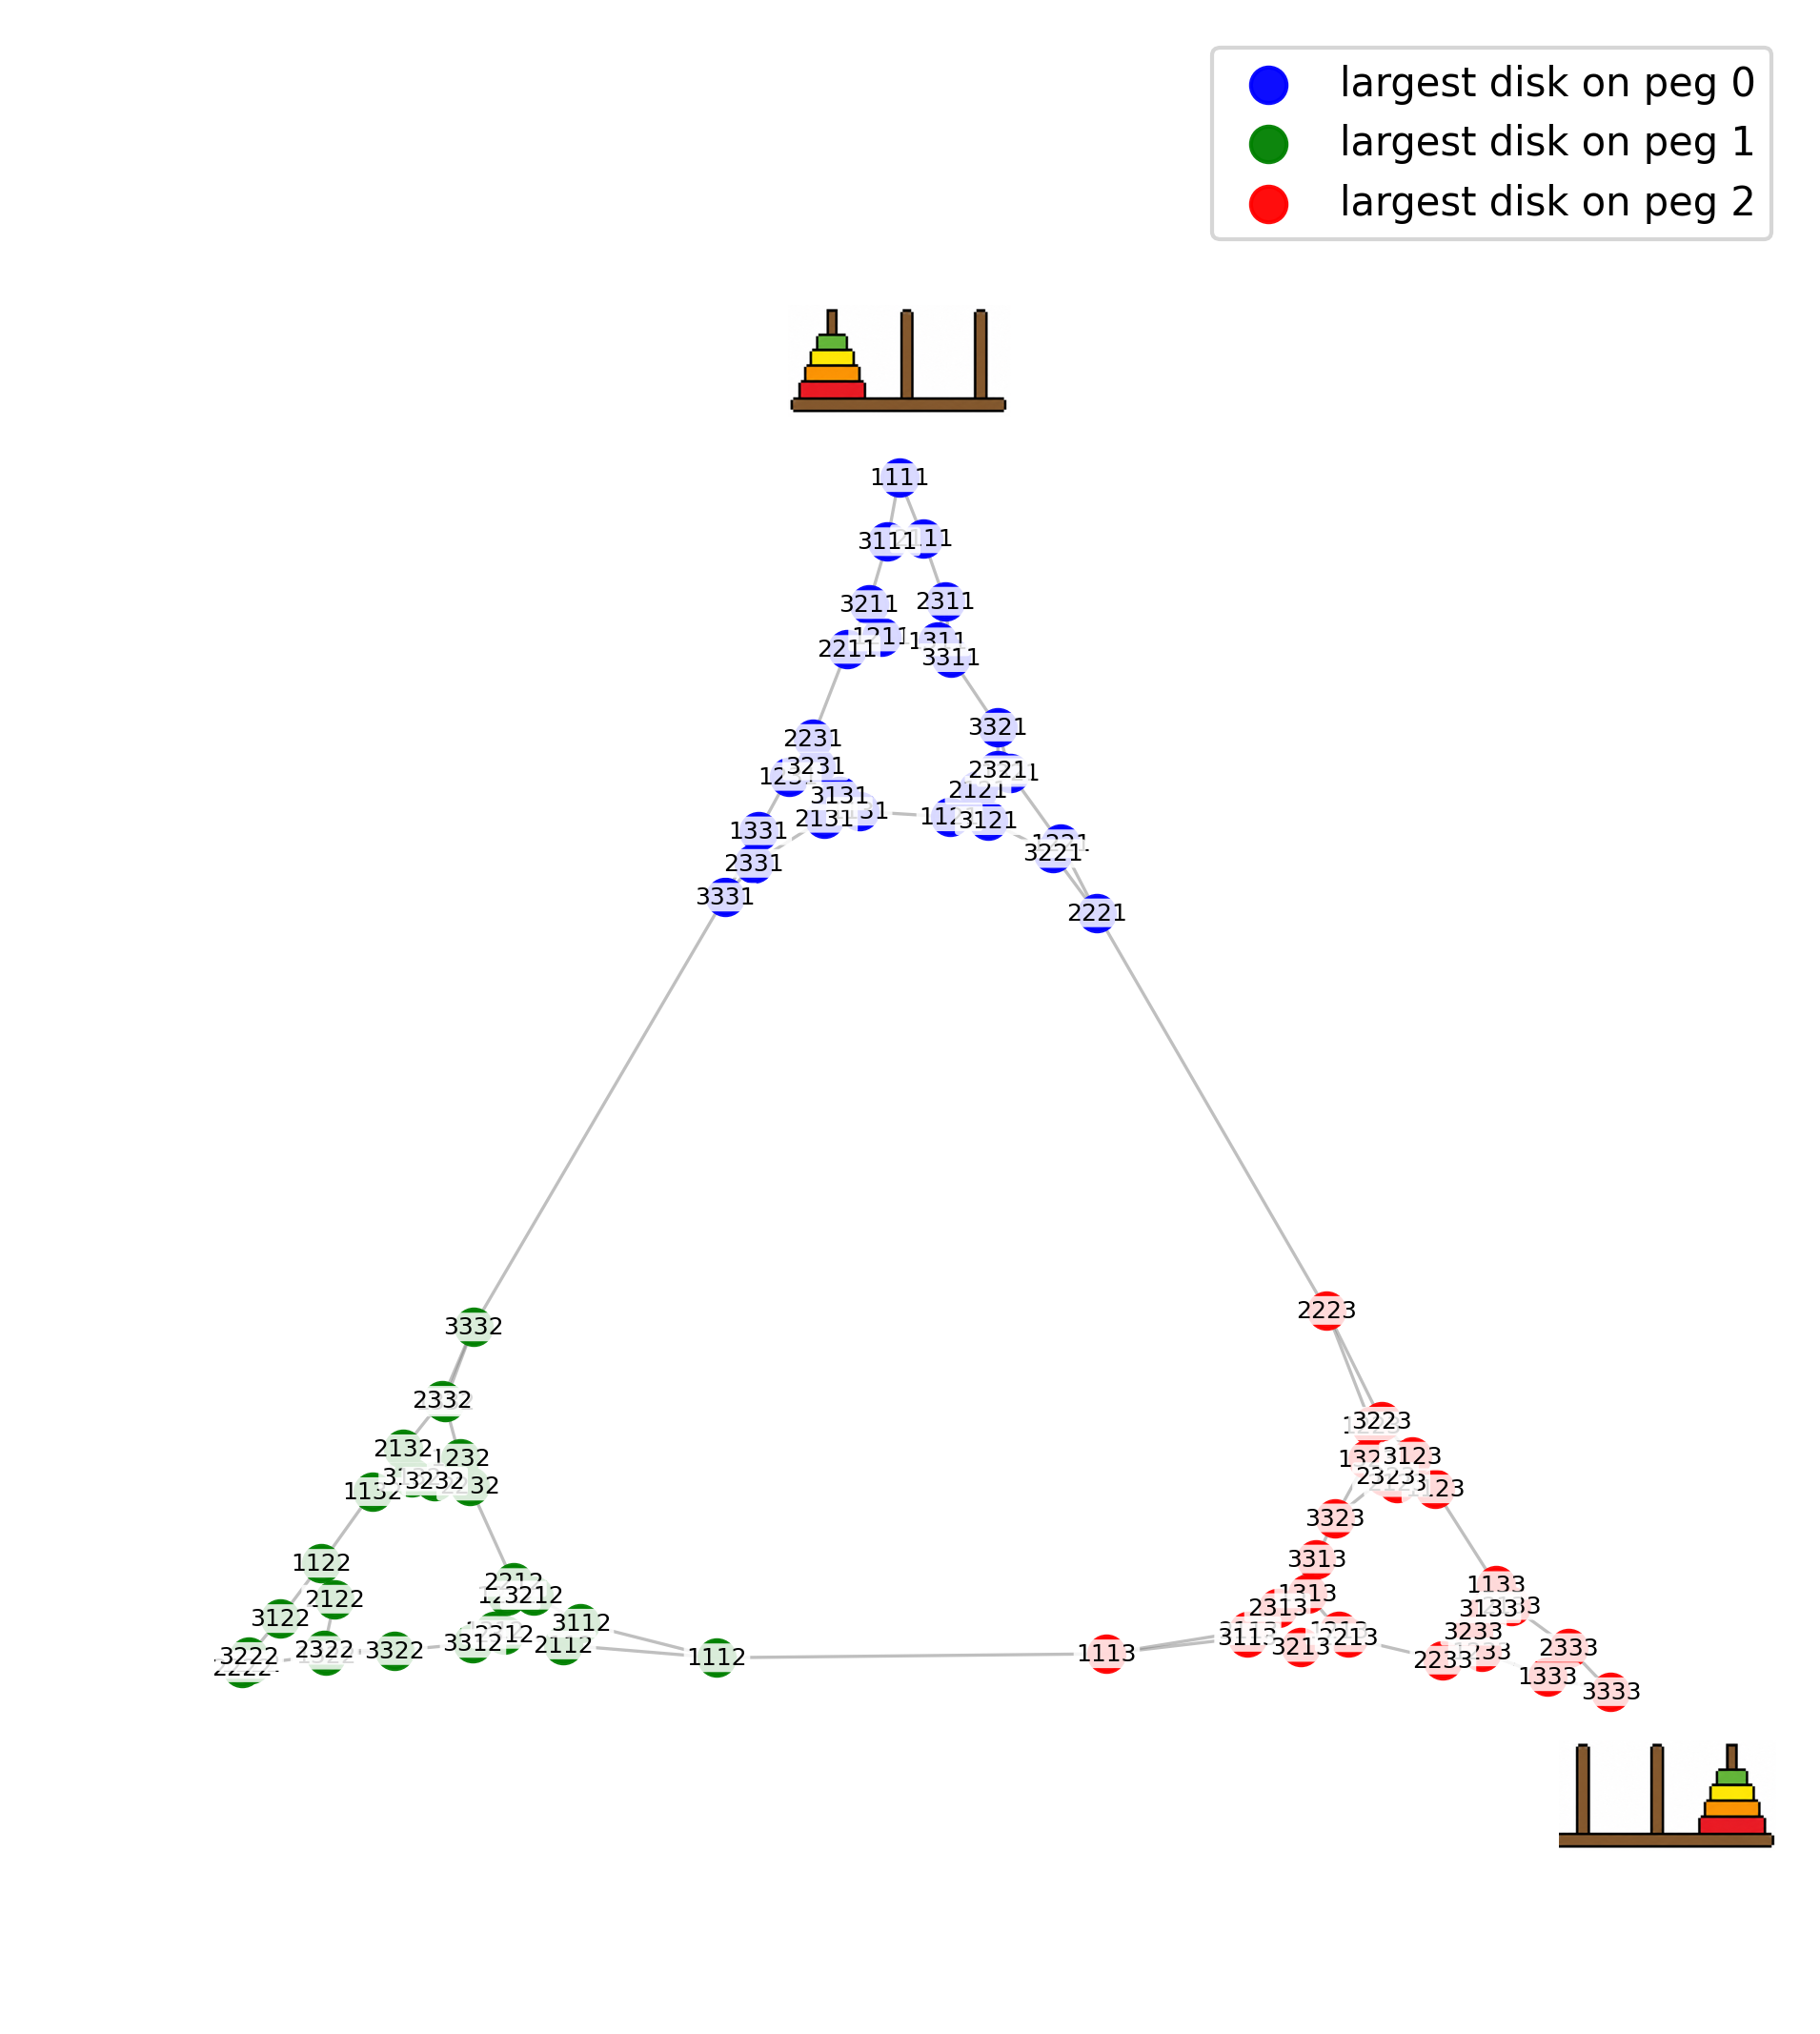
\includegraphics[width=0.5\linewidth]{media/images/probe_sierpinski_epoch50.png}
\caption{2D output of the distance-matching probe on the raw residual stream at layer 5, at epoch 50. Each point is one of the 81 four-disk configurations, coloured by the largest disk's position; grey edges connect graph-adjacent configurations. The three largest-disk sub-triangles separate into the Sierpi\'nski geometry, with cross-cluster gaps wider than the within-cluster edges. Earlier epochs are shown in \Cref{app:probe-2d}.}
\label{fig:sep-probe-epoch50}
\end{figure}

\subsection{A unified-to-factored shift between planning and execution}

Per-disk probes show the state is present at both positions butorganised differently (\Cref{tab:per-disk}). At SEP every disk is recovered perfectly; at move tokens the two small disks remain near-perfect while the larger disks degrade (to $90.7\%$ and $79.3\%$), as the model loses track of infrequently moved disks. Principal angles make the format explicit. Between disk subspaces, they average $54.7^\circ$ at SEP (a \emph{unified}, overlapping encoding that supports the joint Sierpi\'nski geometry) but rise to $76.5^\circ$ at move tokens (a \emph{factored}, near-orthogonal encoding from which each disk can be read independently). The joint distance structure is thus not the sum of the per-disk parts: it lives in the overlapping geometry that the distance probe captures and the per-disk probes discard.

\begin{table}[t]
\centering
\caption{Per-disk classification accuracy (best layer, layer 5). Perfect at SEP; the larger disks degrade at move tokens.}
\label{tab:per-disk}
\begin{tabular}{lrrrrr}
\toprule
\textbf{Position} & \textbf{Disk 0} & \textbf{Disk 1} & \textbf{Disk 2} & \textbf{Disk 3} & \textbf{Mean} \\
\midrule
SEP         & \textbf{100.0\%} & \textbf{100.0\%} & \textbf{100.0\%} & \textbf{100.0\%} & \textbf{100.0\%} \\
Move tokens &  99.98\% &  99.96\% &  90.70\% &  79.25\% &  92.47\% \\
\bottomrule
\end{tabular}
\end{table}

\subsection{The representation is causally used}

Activation patching closes the loop from correlation to causation (\Cref{tab:patching}). Substituting a donor's SEP activation transfers state to the recipient's output in a large majority of pairs. \textsc{Partial} transfer dominates at every layer ($64$--$79\%$), where $K\approx1.45$ of four disks on average are copied from the donor's solution. \textsc{Full} transfer is present ($\sim6\%$), and \textsc{Novel} outcomes are rare ($\leq0.4\%$), so outputs stay tied to donor or recipient. The \textsc{Disrupted} rate falls with depth, from $12.4\%$ at layer 4 to zero at layer 6, i.e. late-layer SEP activations admit clean replacement. The influence is therefore causal but graded, supporting \textbf{H2}.

\begin{table}[t]
\centering
\caption{Activation patching at the SEP token across all donor--recipient validation pairs. \textsc{Partial} transfer dominates; \textsc{disrupted} falls to zero with depth.}
\label{tab:patching}
\begin{tabular}{rrrrrr}
\toprule
\textbf{Layer} & \textbf{Full} & \textbf{Partial (mean $K$)} & \textbf{Unchanged} & \textbf{Novel} & \textbf{Disrupted} \\
\midrule
4 & 5.75\% & 63.89\% ($K{=}1.46$) & 17.56\% & 0.37\% & 12.42\% \\
5 & 6.00\% & 71.77\% ($K{=}1.45$) & 16.49\% & 0.11\% &  5.63\% \\
6 & 5.89\% & 78.74\% ($K{=}1.44$) & 15.37\% & 0.00\% &  0.00\% \\
\bottomrule
\end{tabular}
\end{table}

%==============================================================================
\section{Large reasoning models: emergence, degradation, restoration}
\label{sec:lrm}

\subsection{Flat-to-flat is hard, and depends on reasoning length}
\label{sec:lrm-baselines}

While the standard tower-to-tower task is saturated for current reasoning models (\Cref{app:towertower}), the flat-to-flat formulation is far harder (\Cref{tab:flatflat}). Even the strongest models solve only about half of instances optimally, and accuracy falls steeply with disk count. The final two rows re-evaluate the open-weight models under the much tighter output budget later used for fine-tuning. This isolates how much accuracy depends on reasoning length. Restricting Qwen3.6-27B to that budget collapses its optimal-solve rate from $51\%$ to $14\%$, despite an unchanged Position-A representation: the model that solves half the instances with a mean of $\approx19{,}000$ generated tokens solves a seventh of them when capped. Notably Qwen3.6-27B generates longer traces than DeepSeek-R1-Distill-Qwen-32B on average ($\approx19{,}000$ vs $\approx14{,}000$ tokens), a fact we return to for the steering asymmetry.

\begin{table}[t]
\centering
\caption{Baseline flat-to-flat accuracy (instances solved optimally) on 100 sampled instances per model. \textbf{Max tokens} is the output budget (32k caps the answer only, with provider-side reasoning beyond it; the last two rows use a hard cap: 4096 for $n= \{3, 4$\} and 8192 for $n = 5$).}
\label{tab:flatflat}
\begin{tabular}{lccccc}
\toprule
\textbf{Model} & \textbf{Max tok} & \textbf{3 disks} & \textbf{4 disks} & \textbf{5 disks} & \textbf{Total} \\
\midrule
DeepSeek-R1                  & 32k & 24/34 & 12/33 & 4/33  & 40/100 \\
Kimi-K2-Think                & 32k & 19/34 & 3/33  & 3/33  & 25/100 \\
gpt-oss-120b                 & 32k & 26/34 & 12/33 & 13/33 & \textbf{51/100} \\
\midrule
DeepSeek-R1-Distill-Qwen-32B & 32k & 6/34  & 0/33  & 1/33  & 7/100 \\
Qwen3.6-27B                  & 32k & 28/34 & 14/33 & 9/33  & \textbf{51/100} \\
\midrule
DeepSeek-R1-Distill-Qwen-32B & 4--8k & 14/34 & 1/33 & 0/33 & 15/100 \\
Qwen3.6-27B                  & 4--8k & 8/34  & 2/33 & 4/33 & 14/100 \\
\bottomrule
\end{tabular}
\end{table}

\subsection{Position A: a world model at the end of the prompt}
\label{sec:lrm-posA}

At Position A the distance-matching probe recovers the configuration to essentially perfect accuracy in both models (full per-layer results in \Cref{tab:posA}): from middle depth onward Spearman reaches $0.935$ and nearest-state accuracy $1.00$, identical to the toy SEP token, and the same $\rho{-}r$ asymmetry is preserved. The representation is largely absent at the first layer, but is assembled by layer 8, then plateaus; DeepSeek-R1-Distill-Qwen-32B reaches $\rho=0.936$ with perfect retrieval by middle depth as well. The fact that a 27B pre-trained reasoning model and a 6-layer Transformer trained from scratch encode the configuration with identical fidelity is the strongest evidence that the world model is a property of the task, not of scale or training, extending \textbf{H1} to frontier scale.

\subsection{Positions B and C: degradation through generation}
\label{sec:lrm-posBC}

A faithful prompt-time representation does not translate into a solution. With a maximal reasoning budget, Qwen3.6-27B solves only $51\%$ optimally and the distilled model far fewer. Tracking the probe through generation locates the gap (\Cref{tab:posBC}). At the commitment point (Position B) the joint configuration is not as easily decodable. For Qwen3.6-27B the global geometry is roughly preserved ($\rho\approx0.92$) but nearest-state accuracy drops and the per-disk classifiers collapse to near chance. DeepSeek-R1-Distill-Qwen-32B degrades further on both axes ($\rho$ to $0.74$--$0.81$). During move emission (Position C) the trend of a more factored, per-disk encoding partially returns. This is the large-model counterpart of the toy unified-to-factored shift: a \emph{unified geometry}where planning happens, a \emph{factored} one where execution happens. The degradation appears even on solved problems, therefore maintaining a clean configuration across a long trace is hard even when the model ultimately succeeds, which supports \textbf{H3}.

\begin{table}[t]
\centering
\caption{Probing Qwen3.6-27B through generation. D0--D3 are per-disk probe accuracies.}
\label{tab:posBC}
\begin{tabular}{llrrrrrr}
\toprule
\textbf{Position} & \textbf{Layer} & \textbf{Spearman} & \textbf{Acc} & \textbf{D0} & \textbf{D1} & \textbf{D2} & \textbf{D3} \\
\midrule
A & 24 & \textbf{0.935} & \textbf{1.00} & \textbf{0.75} & \textbf{0.75} & \textbf{0.80} & 0.90 \\
A & 36 & \textbf{0.935} & \textbf{1.00} & 0.59 & 0.69 & 0.75 & \textbf{0.95} \\
A & 48 & \textbf{0.935} & \textbf{1.00} & 0.48 & 0.57 & 0.70 & \textbf{0.95} \\
\midrule
B & 24 & 0.915 & 0.83 & 0.33 & 0.37 & 0.42 & 0.43 \\
B & 36 & 0.915 & 0.75 & 0.33 & 0.33 & 0.41 & 0.34 \\
B & 48 & 0.920 & 0.82 & 0.34 & 0.36 & 0.42 & 0.43 \\
\midrule
C & 24 & 0.802 & 0.41 & \textbf{0.80} & 0.70 & 0.75 & 0.89 \\
C & 36 & 0.813 & 0.64 & 0.58 & 0.62 & 0.60 & 0.84 \\
C & 48 & 0.847 & 0.69 & 0.49 & 0.58 & 0.55 & 0.78 \\
\bottomrule
\end{tabular}
\end{table}

\subsection{Restoring the world model recovers performance}
\label{sec:lrm-steering}

If world model degradation is the bottleneck, restoring the clean Position-A representation at move-emission positions should help. For Qwen3.6-27B it does (\Cref{tab:steering}). Steering is applied only to the problems the model fails unaided. Even the weakest setting converts $44\%$ of failures into optimal solutions. At the best strength ($\alpha=5$), it lifts the optimal-solve count on the 81 configurations from $33$ ($41\%$) to $63$ ($78\%$). The effect is non-monotonic in $\alpha$, i.e. too large a value destabilises generation. The residual failures are rule-violating moves, not parse errors: well-formed but wrong. This is direct causal evidence that the degraded world model limits the model, supporting \textbf{H3}.

For DeepSeek-R1-Distill-Qwen-32B the same intervention does very little: the outcome distribution is identical across every $\alpha$, and even an extreme value ($\alpha = 500$, verified large enough to flip the output logit) yields only parse errors and illegal moves. The natural explanation is output format: DeepSeek-R1-Distill-Qwen-32B frequently fails to emit a parseable move list at all ($35$ of $70$ outputs), so a large share of its failures occur at a stage a state-restoring nudge cannot reach.

\begin{table}[t]
\centering
\caption{Activation steering at layer 36, on the problems each model fails unaided (Qwen: $N{=}48$; DeepSeek: $N{=}70$).}
\label{tab:steering}
\setlength{\tabcolsep}{5pt}
\begin{tabular}{llrrrr}
\toprule
\textbf{Model} & \textbf{$\alpha$} & \textbf{Optimal} & \textbf{Suboptimal} & \textbf{Incorrect} & \textbf{Illegal} \\
\midrule
\multirow{5}{*}{Qwen3.6-27B} & 0.5 & 21 & 10 & 1 & 16 \\
 & 1  & 22 & 6  & 3 & 17 \\
 & 2  & 18 & 13 & 1 & 16 \\
 & 5  & \textbf{30} & 5  & 3 & 10 \\
 & 10 & 21 & 5  & 5 & 17 \\
\midrule
DeepSeek-R1-Distill-Qwen-32B & 0.5--10 & 2 & 2 & 1 & 65 \\
\bottomrule
\end{tabular}
\end{table}

\subsection{Restoration in the weights: a state-encoding loss}
\label{sec:lrm-finetune}

\begin{figure}[H]
\centering
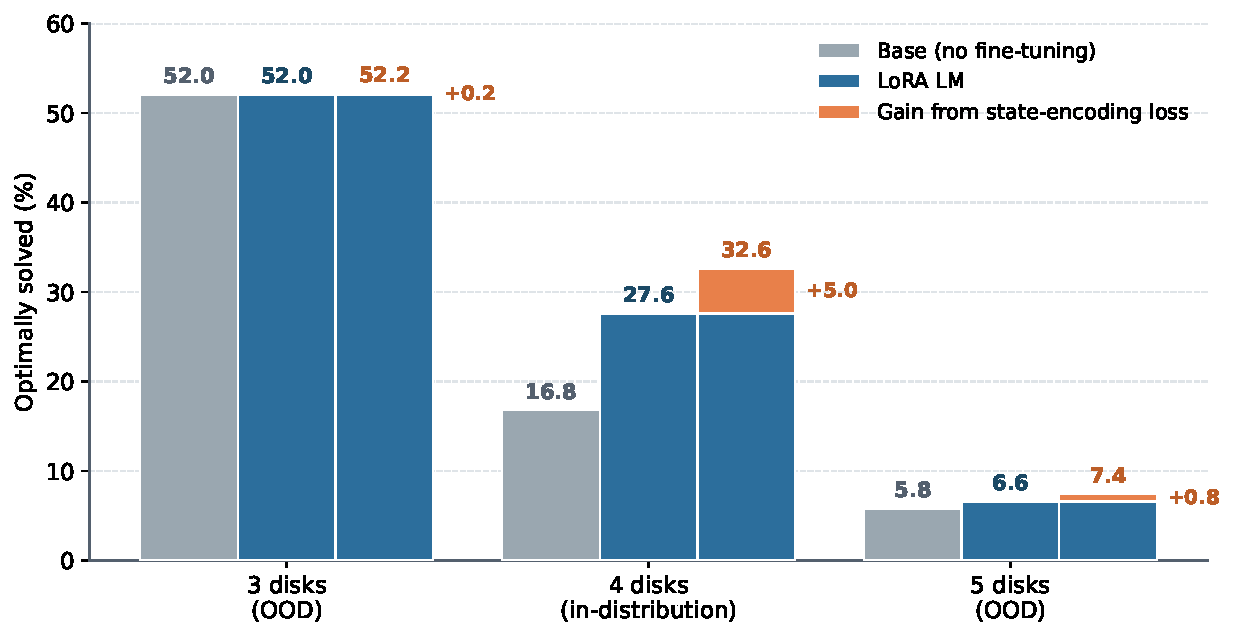
\includegraphics[width=0.58\linewidth]{media/images/finetune_optimal.pdf}
\caption{Optimally solved problems for Qwen3.6-27B: the base model with no fine-tuning (grey), and after one epoch of LoRA fine-tuning under the language-modelling baseline vs.\ the added state-encoding loss (layer 36, $\alpha=0.2$). The coral segment is the gain from the state-encoding loss. $n=4$ is in-distribution; $n=3,5$ are out-of-distribution.}
\label{fig:finetune}
\end{figure}

We apply the same correction into the weights using a LoRA adapter as an auxiliary state-encoding loss (\Cref{sec:method-lrm}); it improves the optimal-solve count at every disk count over a language-modelling-only baseline, on $500$ held-out problems per disk count (\Cref{fig:finetune}): the largest gain is in-distribution ($n=4$: $138\to163$) at no cost out-of-distribution ($n=3$: $260\to261$; $n=5$: $33\to37$). Where steering is an inference-time control, here the same direction serves as a training signal that strengthens the state encoding into the weights, removing the need for any external state-tracker at deployment.


%==============================================================================
\section{Discussion}
\label{sec:discussion}

The two streams lead to one narrative: a geometrically structured world model emerges by the end of the prompt in models separated by orders of magnitude in size, degrades over the course of generation, and recovers solution accuracy when restored, at inference or in the weights.

\paragraph{An emergent, causal world model that is not an artifact of scale.}
The distance-matching probe recovers the joint configuration, and reproduces the Sierpi\'nski geometry of the state graph, at the toy SEP token and at the final prompt token of both frontier models with near-identical fidelity, down to the shared Spearman--Pearson gap that signals inflated separation between the largest-disk sub-triangles (\Cref{tab:sep-probe,tab:posA}). That a 6-layer Transformer trained from scratch and a 27B reasoning model encode the state alike argues the world model is a property of the task, not of scale or training regime. We extend the emergent-world-model line~\citep{li2022emergent, toshniwal2022chess, spies2025transformers} from one-move-per-pass game settings into planning solved through extended chain-of-thought. Activation patching closes the loop from correlation to causation. Substituting a donor's SEP activation transfers state to the recipient's output in a large majority of pairs (\Cref{tab:patching}), so the representation is read, not merely present. 

\paragraph{Degradation through generation reframes the collapse.}
A faithful prompt-time representation does not yield a solution: both models recover the state near-perfectly at Position A yet solve only about half of flat-to-flat instances optimally (\Cref{tab:flatflat,tab:posBC}). Tracking the probe through generation locates the gap, the joint configuration becomes hard to read at the commitment point and a more factored, per-disk encoding partially returns during emission, the large-model counterpart of the toy unified-to-factored shift. This sharpens \citet{shojaee2025illusion}: the collapse is, at least in part, a failure to maintain a representation the model demonstrably had, not the absence of one. Restoring the clean Position-A activation at move-emission positions nearly doubles Qwen3.6-27B's optimal-solve count (\Cref{tab:steering}), direct causal evidence that the degraded world model is the bottleneck. As in Othello-GPT~\citep{li2022emergent}, the steered model acts on the injected configuration, emitting well-formed move lists with no format errors at any $\alpha$; its residual failures are illegal \emph{moves}, not malformed output. Folding the same direction into a LoRA adapter as an auxiliary state-encoding loss improves accuracy at every disk count, largest in-distribution and at no out-of-distribution cost (\Cref{fig:finetune}).

\paragraph{Steering does not transfer}
The intervention does essentially nothing for DeepSeek-R1-Distill-Qwen-32B, despite its near-identical Position-A probe (\Cref{tab:steering}). The cleaner differentiator between the two models is output format, DeepSeek frequently emits no parseable move list at all, so many failures occur where a state-restoring nudge cannot reach. A representational mismatch, the load-bearing layer-36 direction for Qwen not being DeepSeek's own state code at emission, remains possible; separating the two is the most important open question we leave to future work.

\paragraph{Limitations.}
Experiments use a single puzzle at a single size ($n{=}4$), with only small out-of-distribution checks at $n{=}3,5$; Tower of Hanoi's clean recursive structure is what makes its graph a convenient probe target. Whether the story of emergence then degradation, and finally restoration, holds for less geometric state spaces is untested. The two frontier models are both Qwen-derived, so transfer should be read within that caveat. A supervised probe can fit structure the model does not use, we mitigate this with patching and steering, which test causal use directly. Several figures rest on single seeds, and the state-encoding loss was evaluated at one hyperparameter setting (layer band, $\alpha$, auxiliary weight), so its gains are a lower bound. The steering method also relies on an external state-tracker that recomputes the true state after each move, feasible here but not obviously scalable to tasks where ground-truth state is expensive or ambiguous. The fine-tuning and steering runs also used a constrained output-token budget for tractability; since flat-to-flat accuracy depends on reasoning length (\Cref{tab:flatflat}), the reported solve rates and the steering and fine-tuning gains are likely conservative. Finally, the technique that restores a correct world model could steer one toward a non-benign target, a capability whose governance deserves attention as such methods mature.

%==============================================================================
\section{Conclusion}
\label{sec:conclusion}

We asked where a reasoning model's planning failure lives, and found it is neither an absent world model nor a pure decoding fault but a failure to maintain a representation the model demonstrably forms. A linear distance-matching probe recovers the Tower of Hanoi configuration, in faithful Sierpi\'nski geometry. We find this structure in a toy Transformer's SEP token and in the final prompt token of two frontier reasoning models alike (H1). Activation patching shows the toy representation is causally read rather than merely present (H2). Furthermore, tracking the probe through generation shows the frontier representation is near-perfect at the end of the prompt, degrades at the commitment point, and returns only in factored form during emission (H3). Restoring it, either by steering at inference or through an auxiliary state-encoding loss in the weights, recovers much of the lost accuracy for Qwen3.6-27B, though not for DeepSeek-R1-Distill-Qwen-32B, whose unparseable outputs leave the intervention nothing to correct. The reported collapse is thus better read as the model forgetting what it knew than as an inability to represent the problem, a reframing that points mitigation toward maintaining state across a long trace rather than toward more inference-time search.

\bibliography{references}
\bibliographystyle{colm2026_conference}

\appendix
\section{Unsupervised dimensionality reduction}
\label{app:unsup}
As a probe-free check, SEP-token activations for all 81 start states (fixed goal) were projected to 2D with PCA, t-SNE, and UMAP at every layer (\Cref{fig:dimred}). None of the eighteen panels reproduces the Sierpi\'nski geometry; at best a coarse grouping by the largest disk's position emerges. The model does not store the state space in a representation whose \emph{raw} projected geometry is Sierpi\'nski-like, motivating the supervised distance-matching probe.

\begin{figure}[h]
\centering
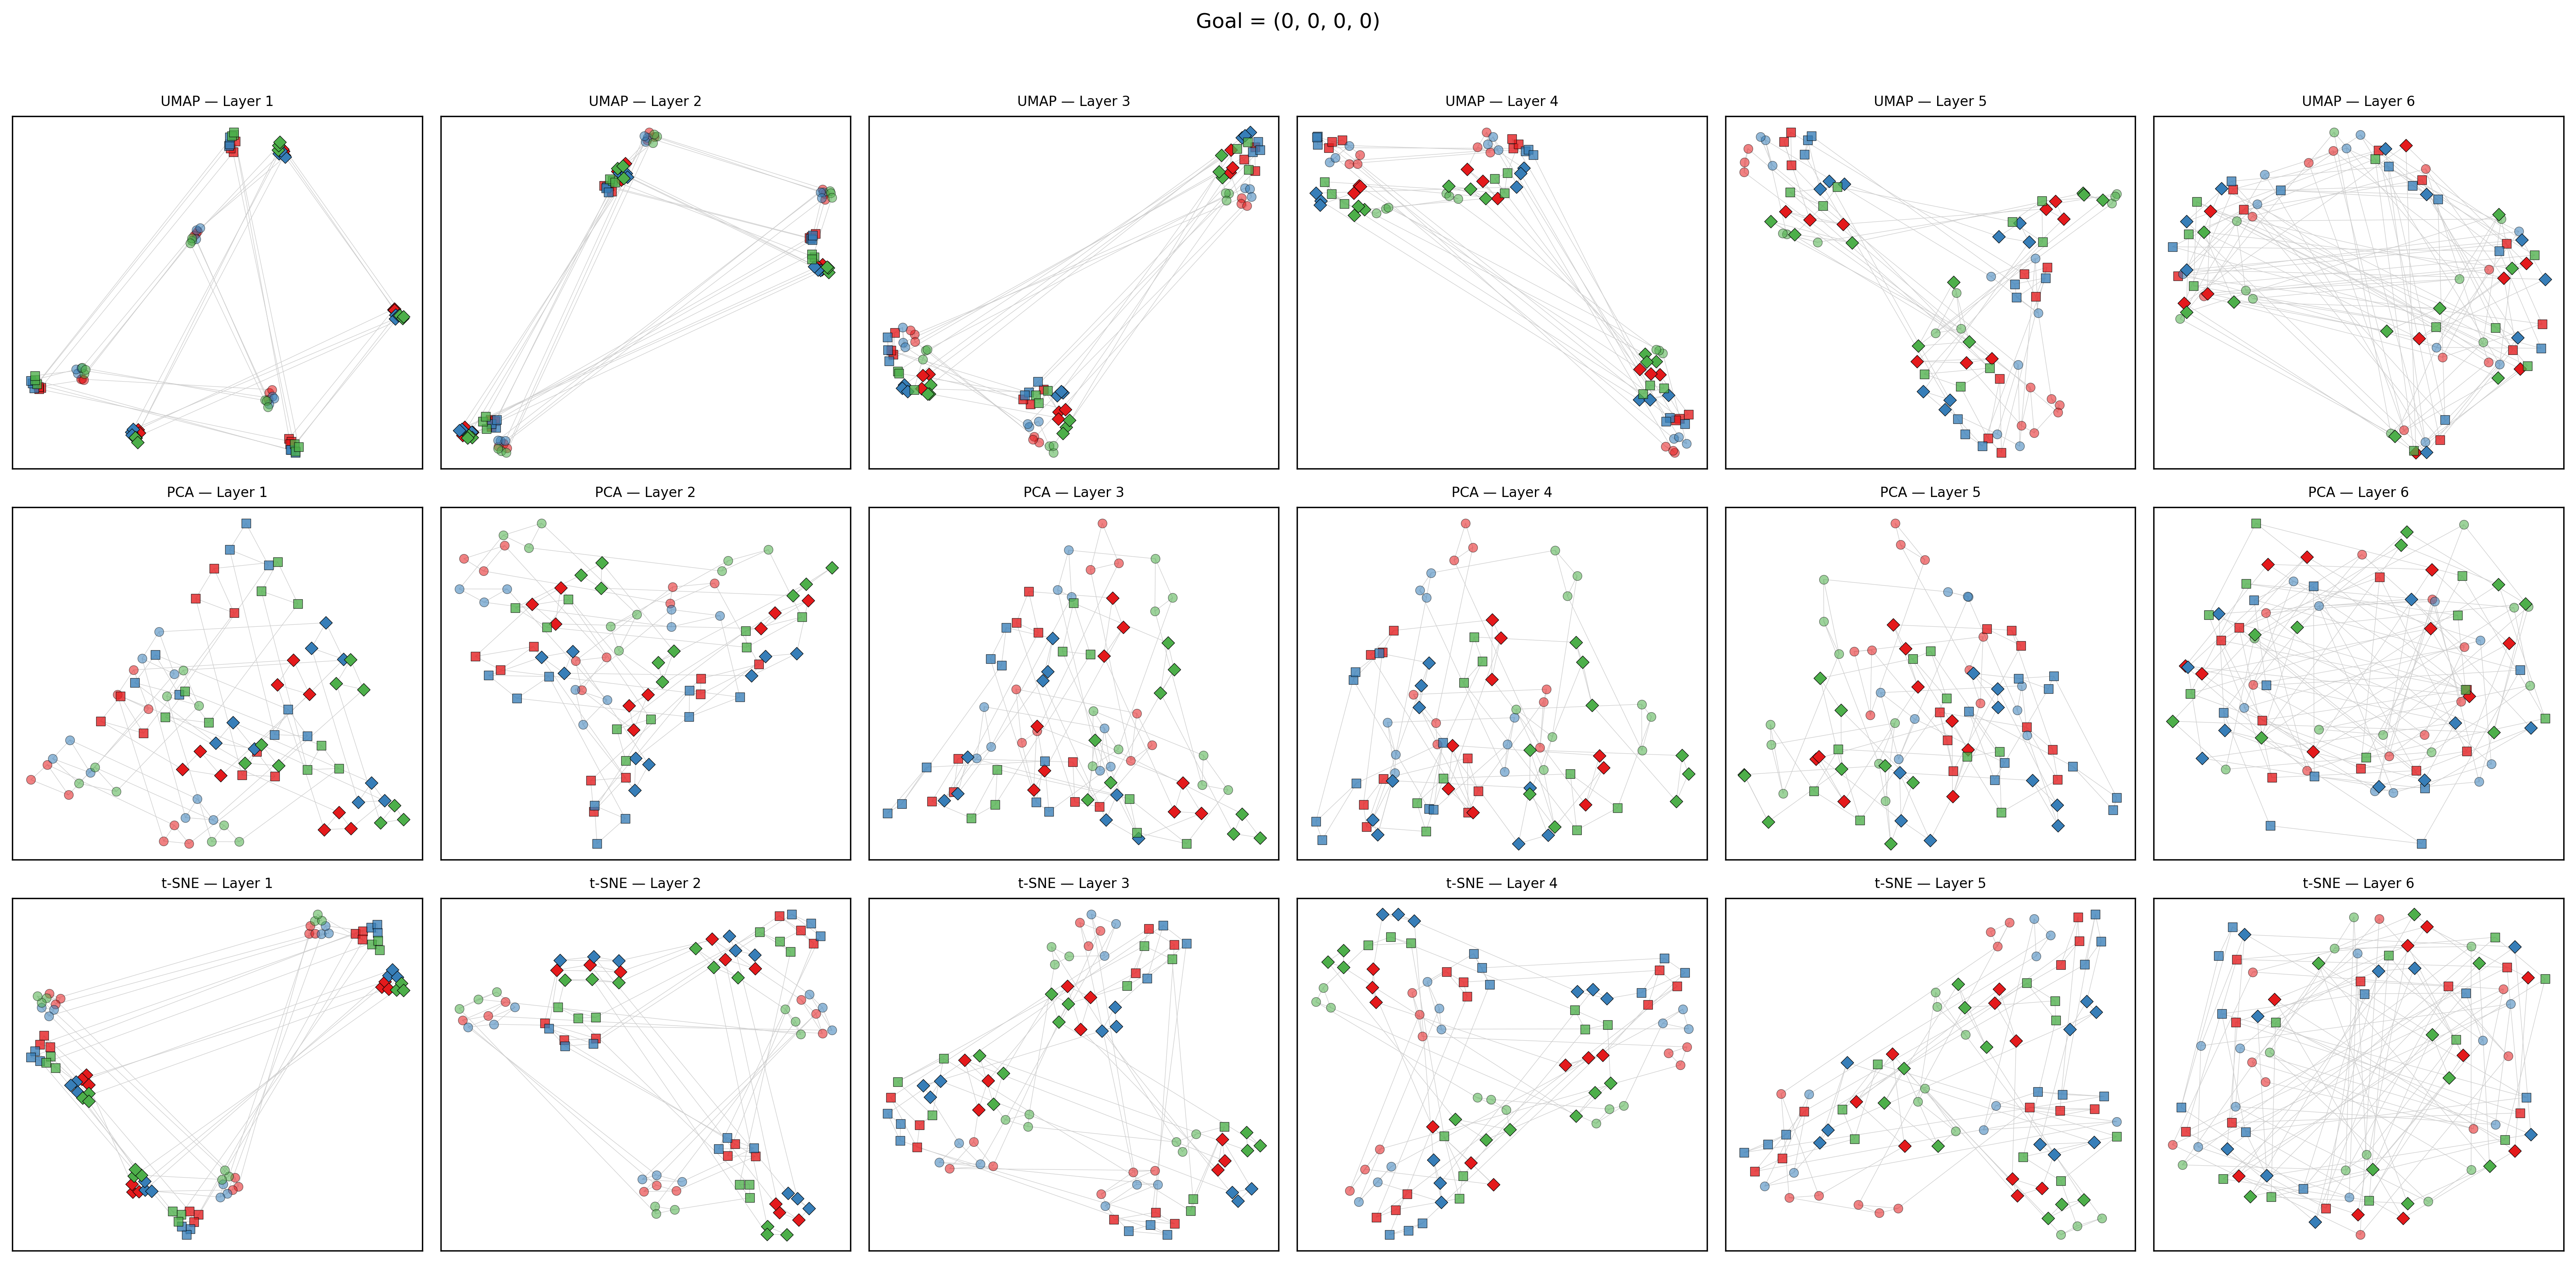
\includegraphics[width=\linewidth]{media/images/toy_dimred_grid.png}
\caption{Two-dimensional projections of SEP-token hidden states across the three techniques (rows) and six layers (columns), coloured by largest-disk position. No panel recovers the Sierpi\'nski structure.}
\label{fig:dimred}
\end{figure}

\section{Probe geometry over training}
\label{app:probe-2d}
\begin{figure}[h]
\centering
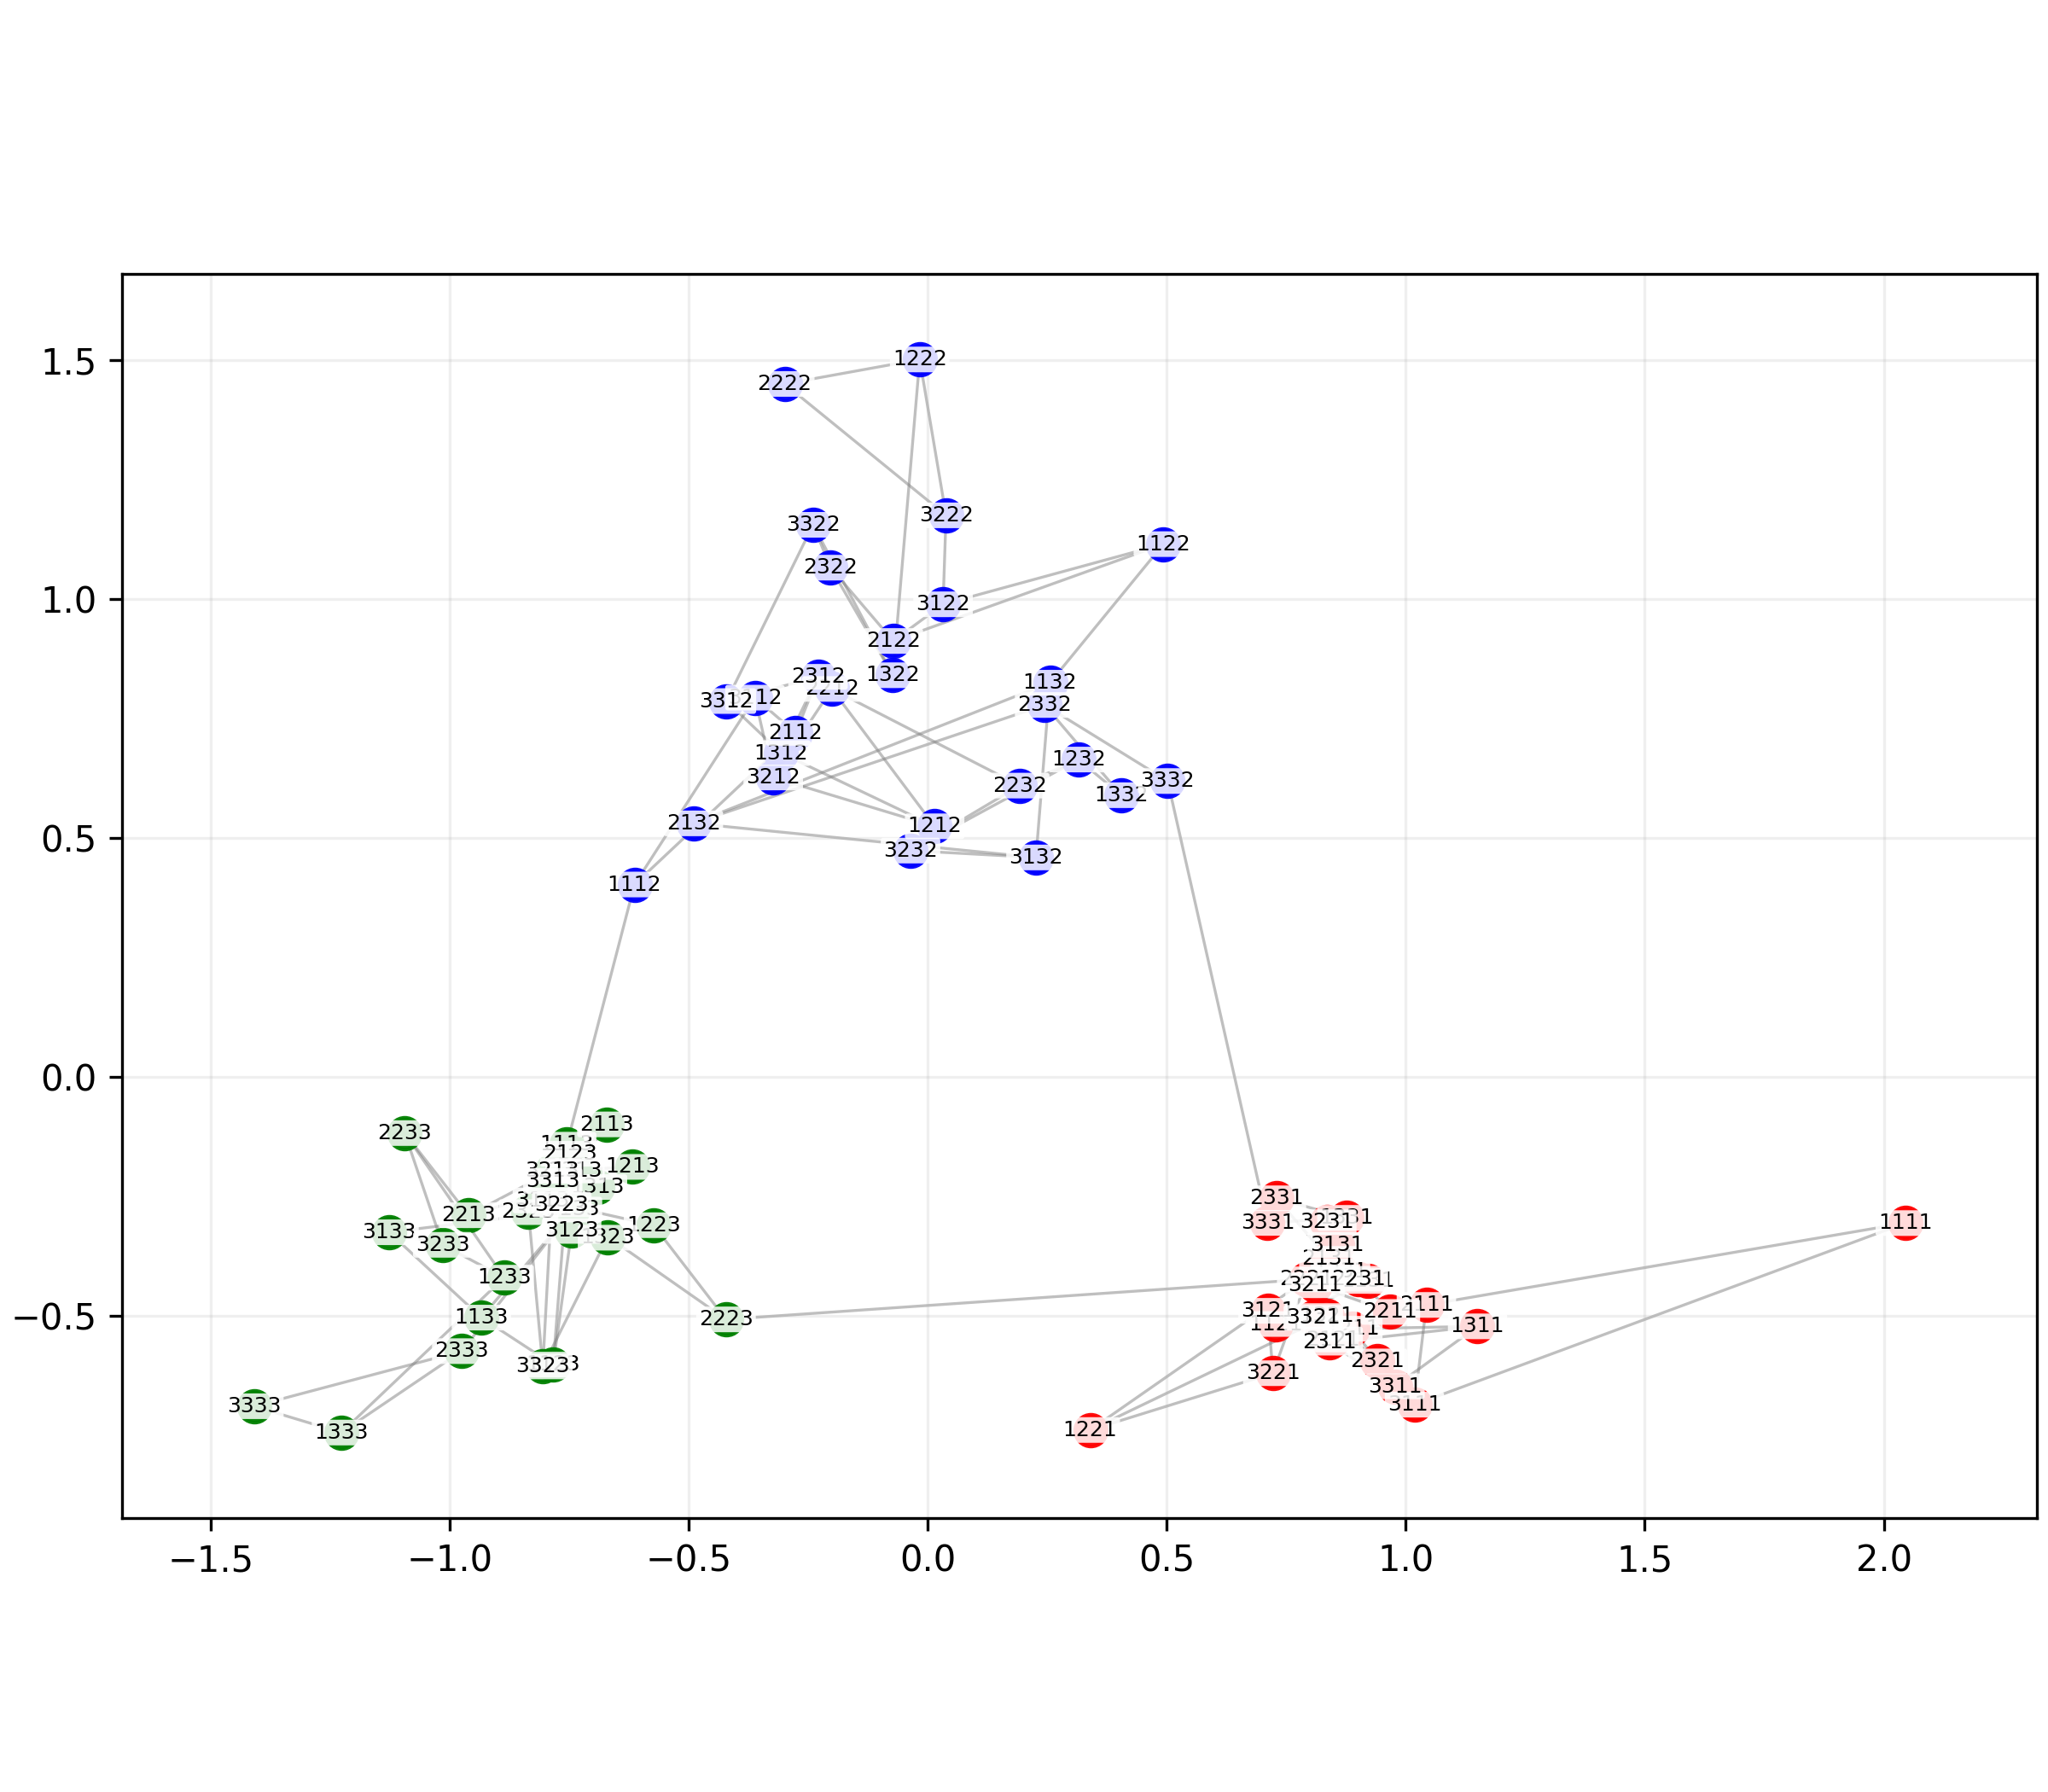
\includegraphics[width=0.32\linewidth]{media/images/probe_sierpinski_epoch05.png}\hfill
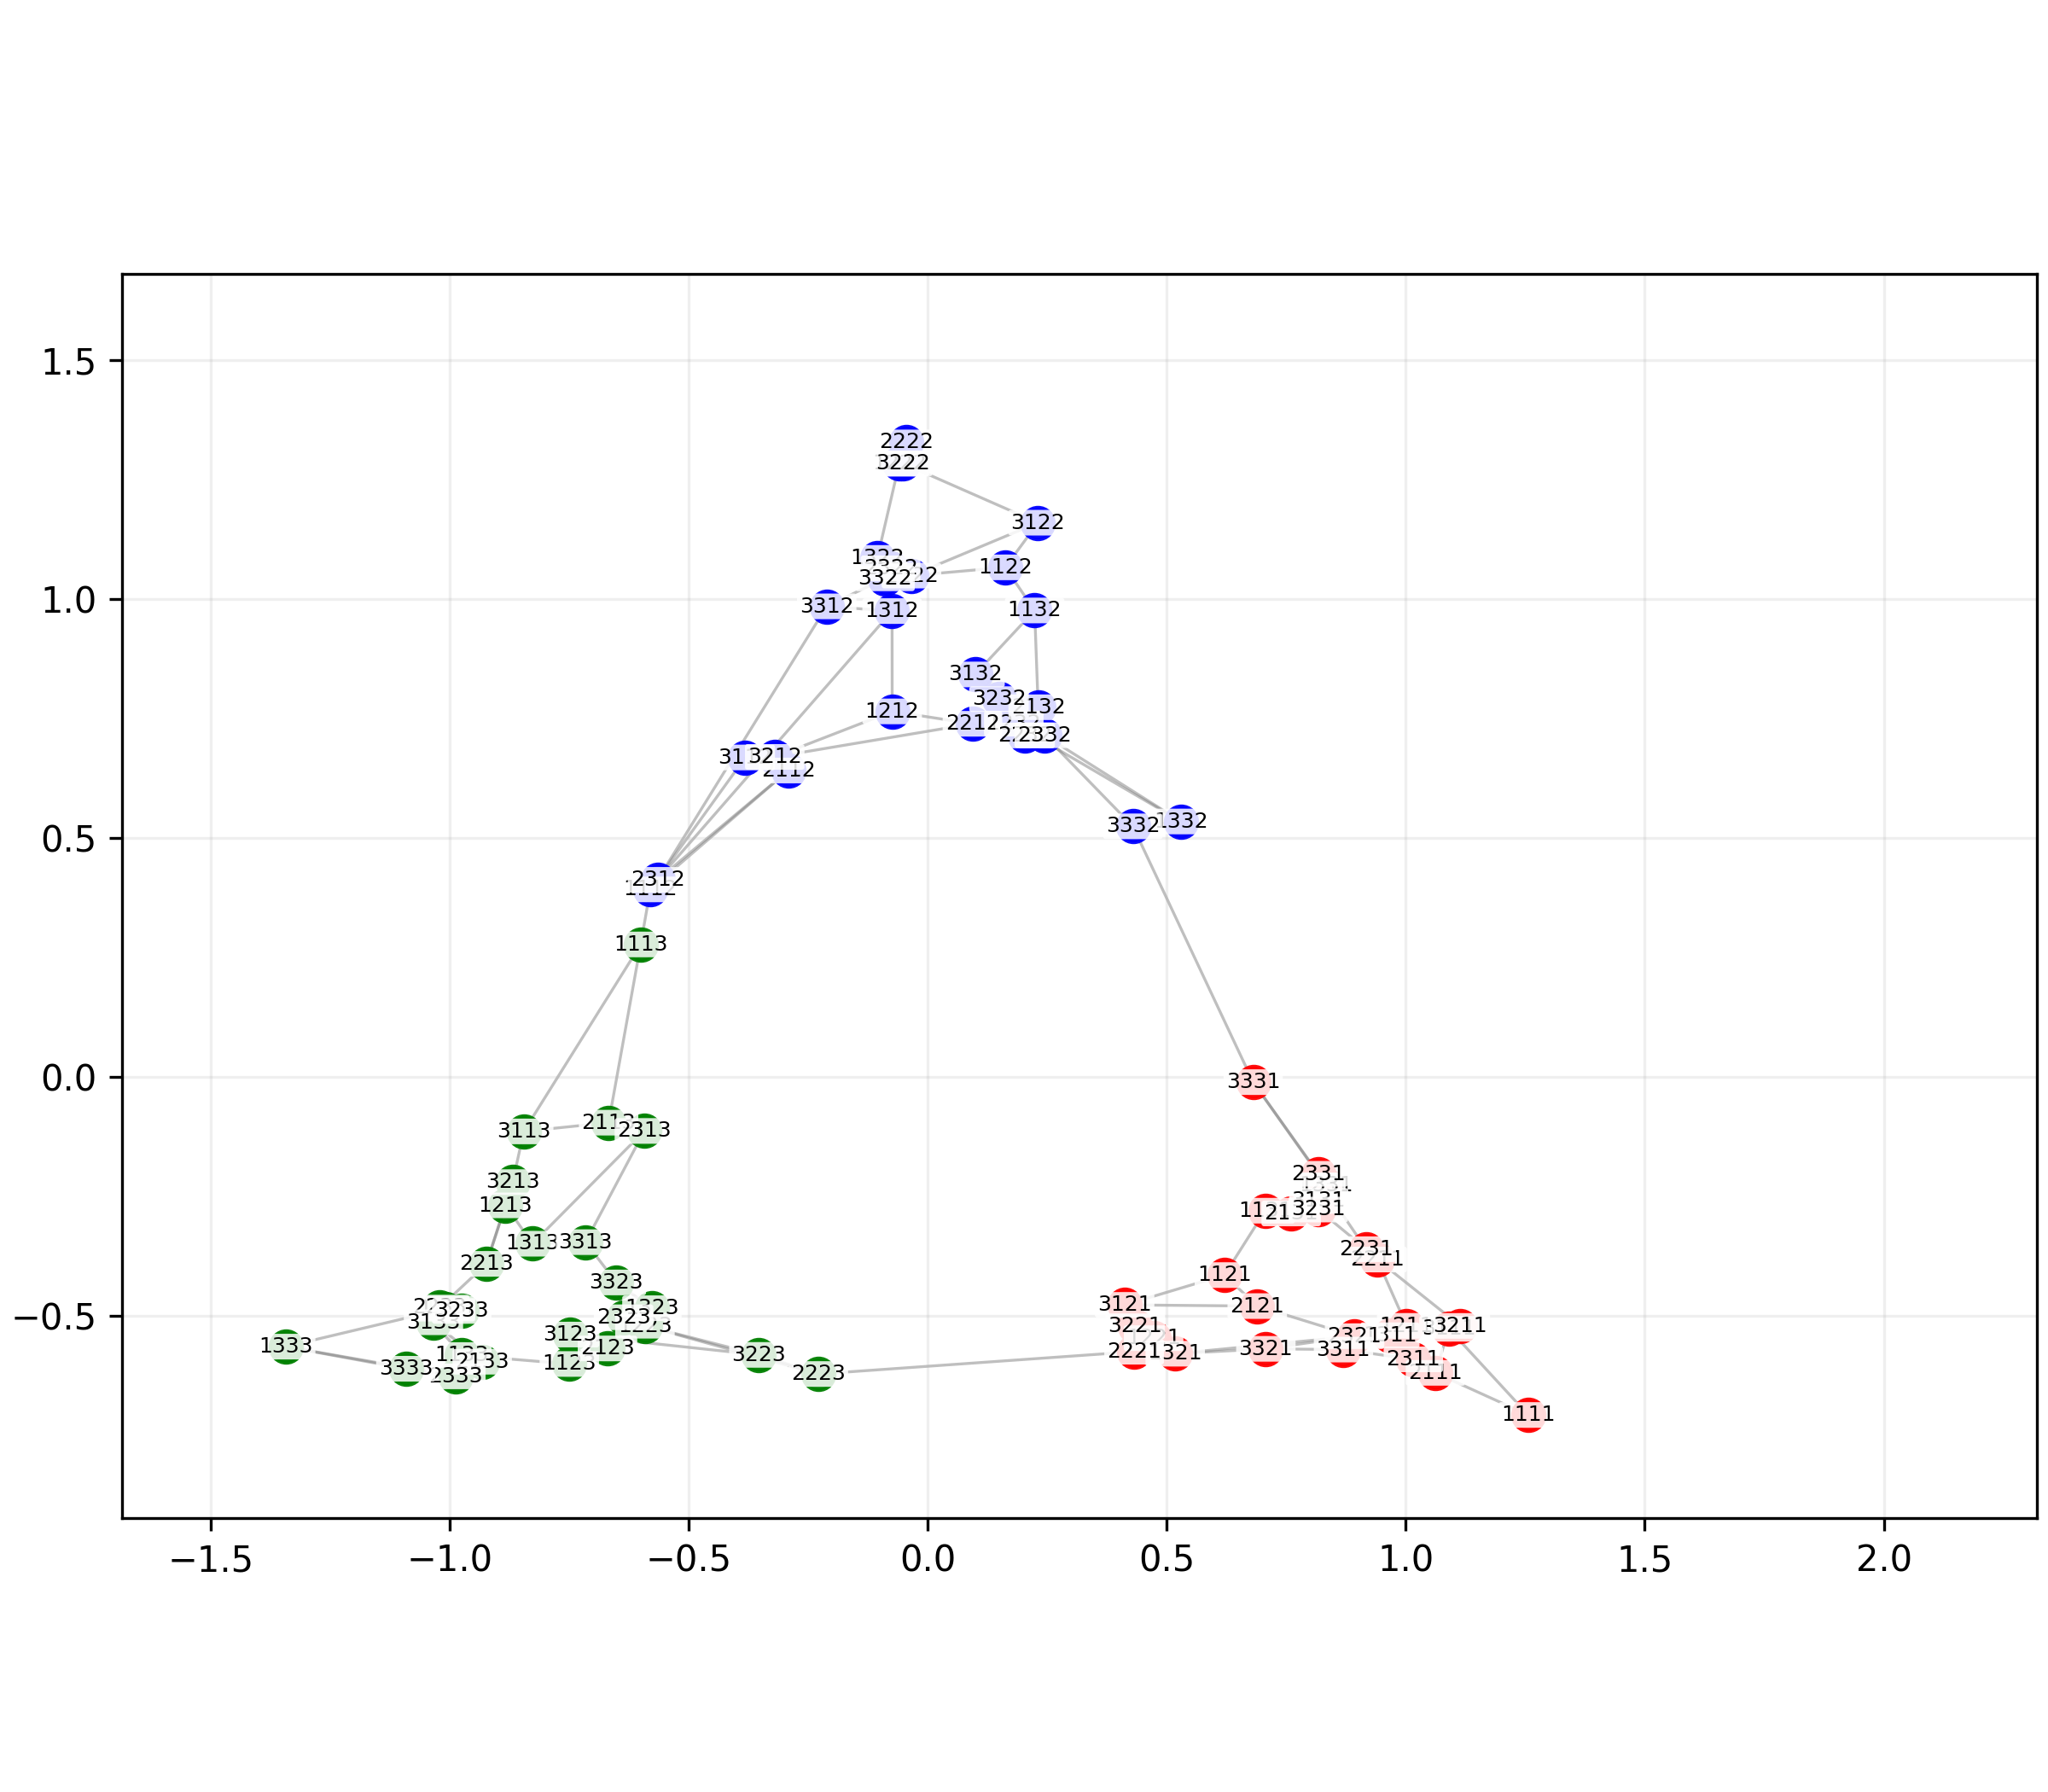
\includegraphics[width=0.32\linewidth]{media/images/probe_sierpinski_epoch25.png}\hfill
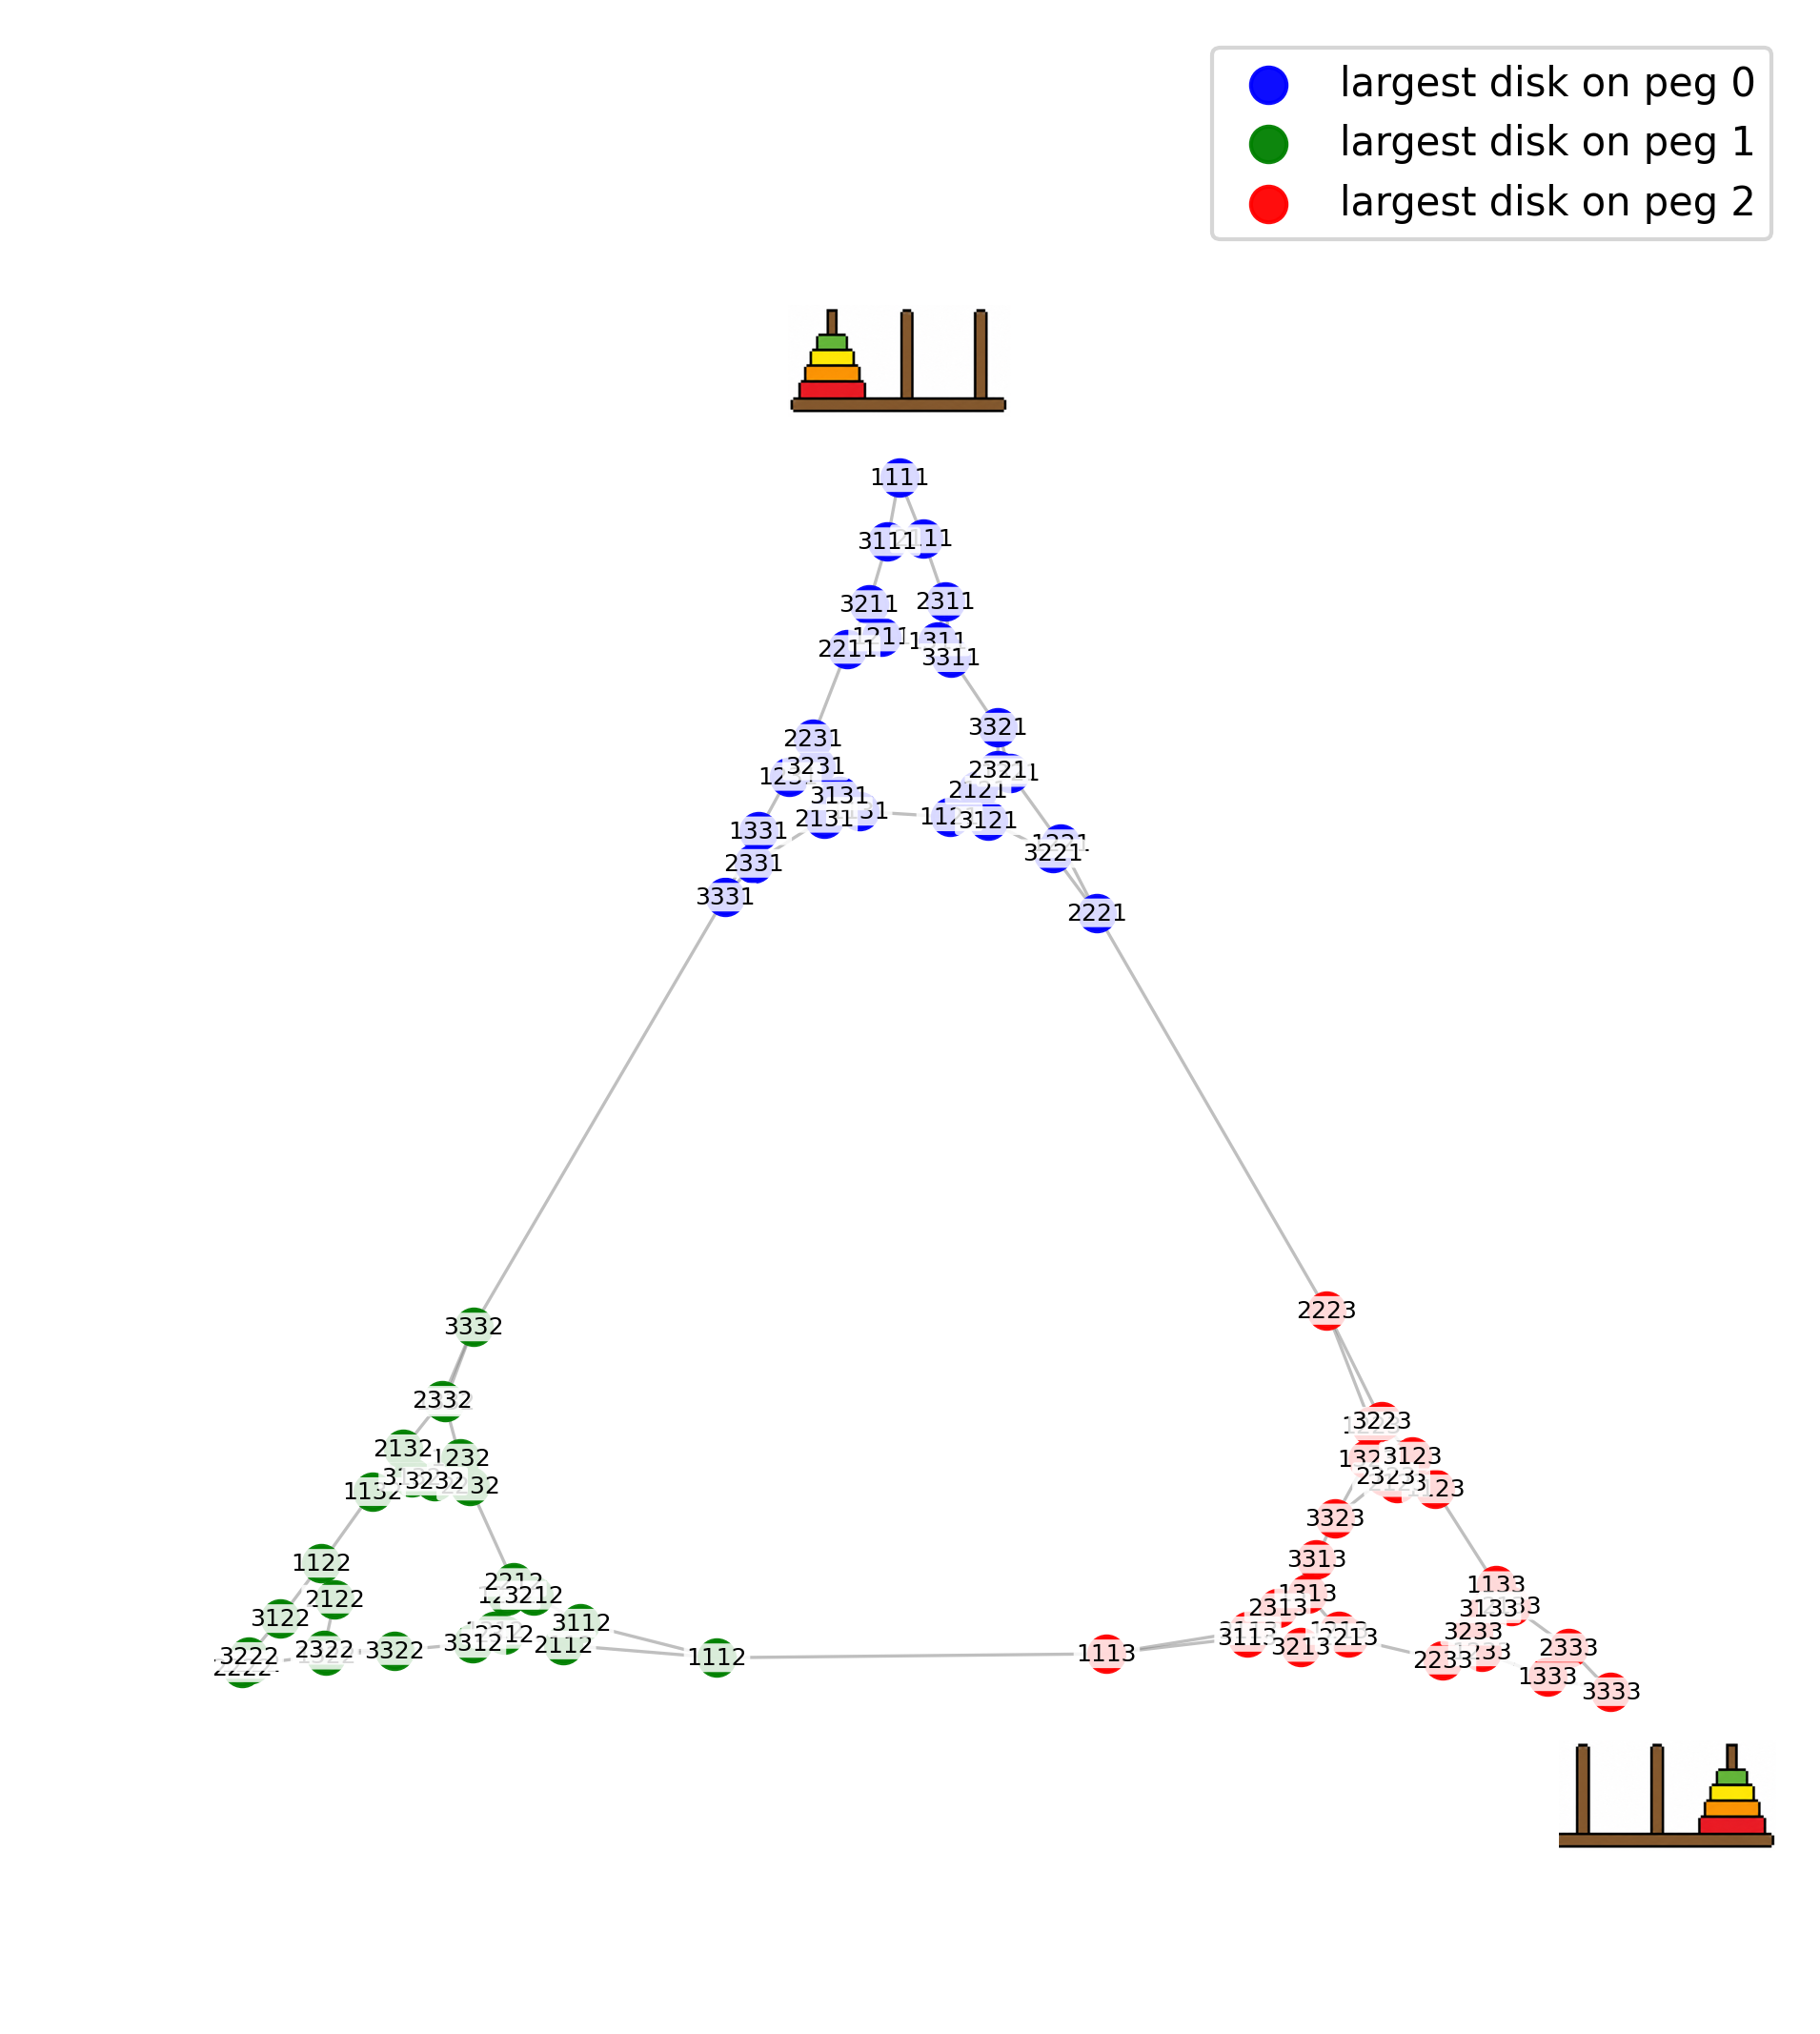
\includegraphics[width=0.32\linewidth]{media/images/probe_sierpinski_epoch50.png}
\caption{2D output of the distance-matching probe at layer 5 over training (epochs 5, 25, 50). The Sierpi\'nski structure sharpens as the three largest-disk sub-triangles separate.}
\label{fig:probe-2d}
\end{figure}

\section{Move-token probes}
\label{app:move-probes}
The joint state is not recoverable from individual move-token activations. Across four probe variants the best result is a 15-token multi-position window at $\rho=0.781$ and $7.6\%$ nearest-state accuracy, far below the SEP token's $\rho=0.938$ at $100\%$ retrieval (\Cref{tab:move-probe}).

\begin{table}[h]
\centering
\caption{Best configuration of each move-token probe (selected by Spearman), with the SEP linear probe for reference.}
\label{tab:move-probe}
\begin{tabular}{lrrr}
\toprule
\textbf{Probe} & \textbf{Layer} & \textbf{Nearest-state acc.} & \textbf{Spearman $\rho$} \\
\midrule
Linear (pooled)              & 4 & 1.5\% & 0.295 \\
Per-step controlled          & 3 & 1.0\% & 0.610 \\
Nonlinear (MLP)              & 4 & 4.1\% & 0.668 \\
Multi-position ($K{=}15$)    & 3 & \textbf{7.6\%} & \textbf{0.781} \\
\midrule
SEP token (linear, ref.)     & 5 & 100\%   & 0.938 \\
\bottomrule
\end{tabular}
\end{table}

\section{Sparse autoencoder analysis}
\label{app:sae}
To test whether the move-token state is in superposition, sparse autoencoders were trained on residual-stream activations at layers 4--5 (expansion $\{2,4,8,16\}$, $L^1$ penalty $\lambda\in\{0.5,1,2,4\}$) and the distance probe re-trained on the latents. At SEP the SAE latents and raw activations give nearly identical probe quality ($\rho=0.935$ either way); at move tokens the SAE roughly doubles nearest-state accuracy but absolute values stay very low. The SAE offers no evidence of substantial superposition: the structure the linear probes recover from the raw residual stream is the same structure the SAE recovers (\Cref{fig:sae}).

\begin{figure}[h]
\centering
\begin{minipage}{0.7\textwidth}
\centering
\begin{minipage}{0.48\linewidth}\centering Raw residual\\[2pt]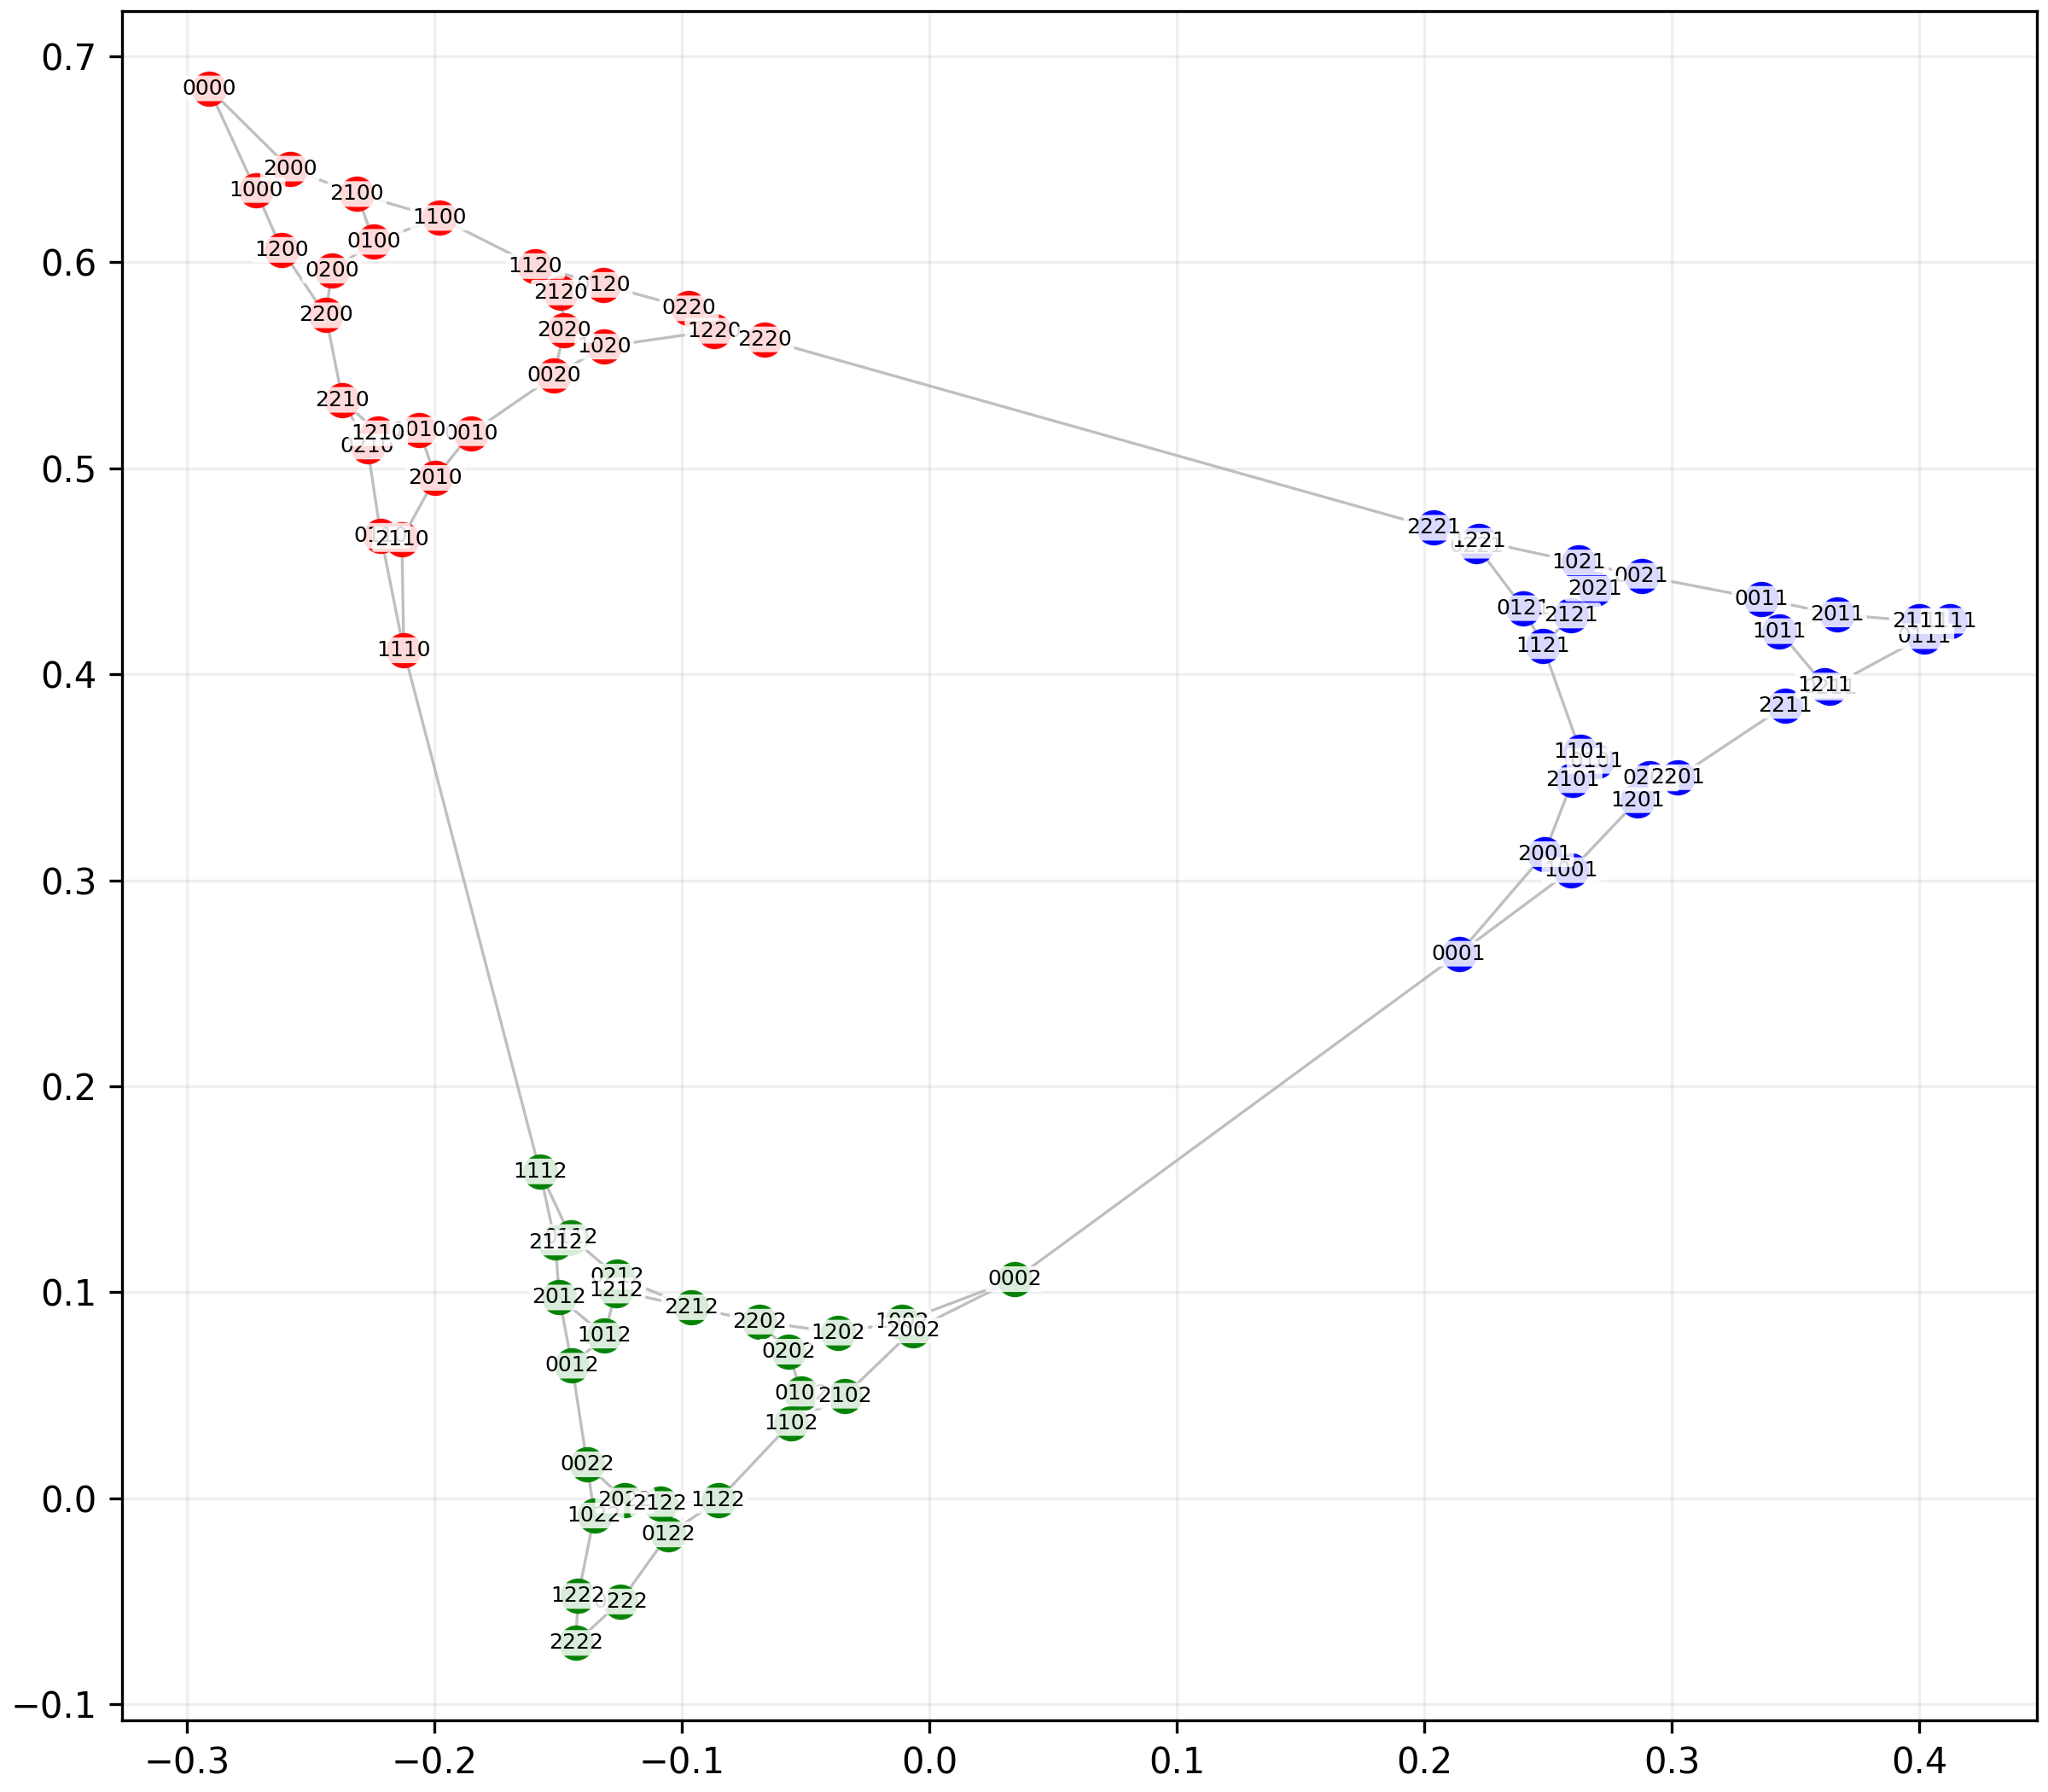
\includegraphics[width=\linewidth]{media/images/sae_sep_raw.png}\end{minipage}\hfill
\begin{minipage}{0.48\linewidth}\centering SAE latent\\[2pt]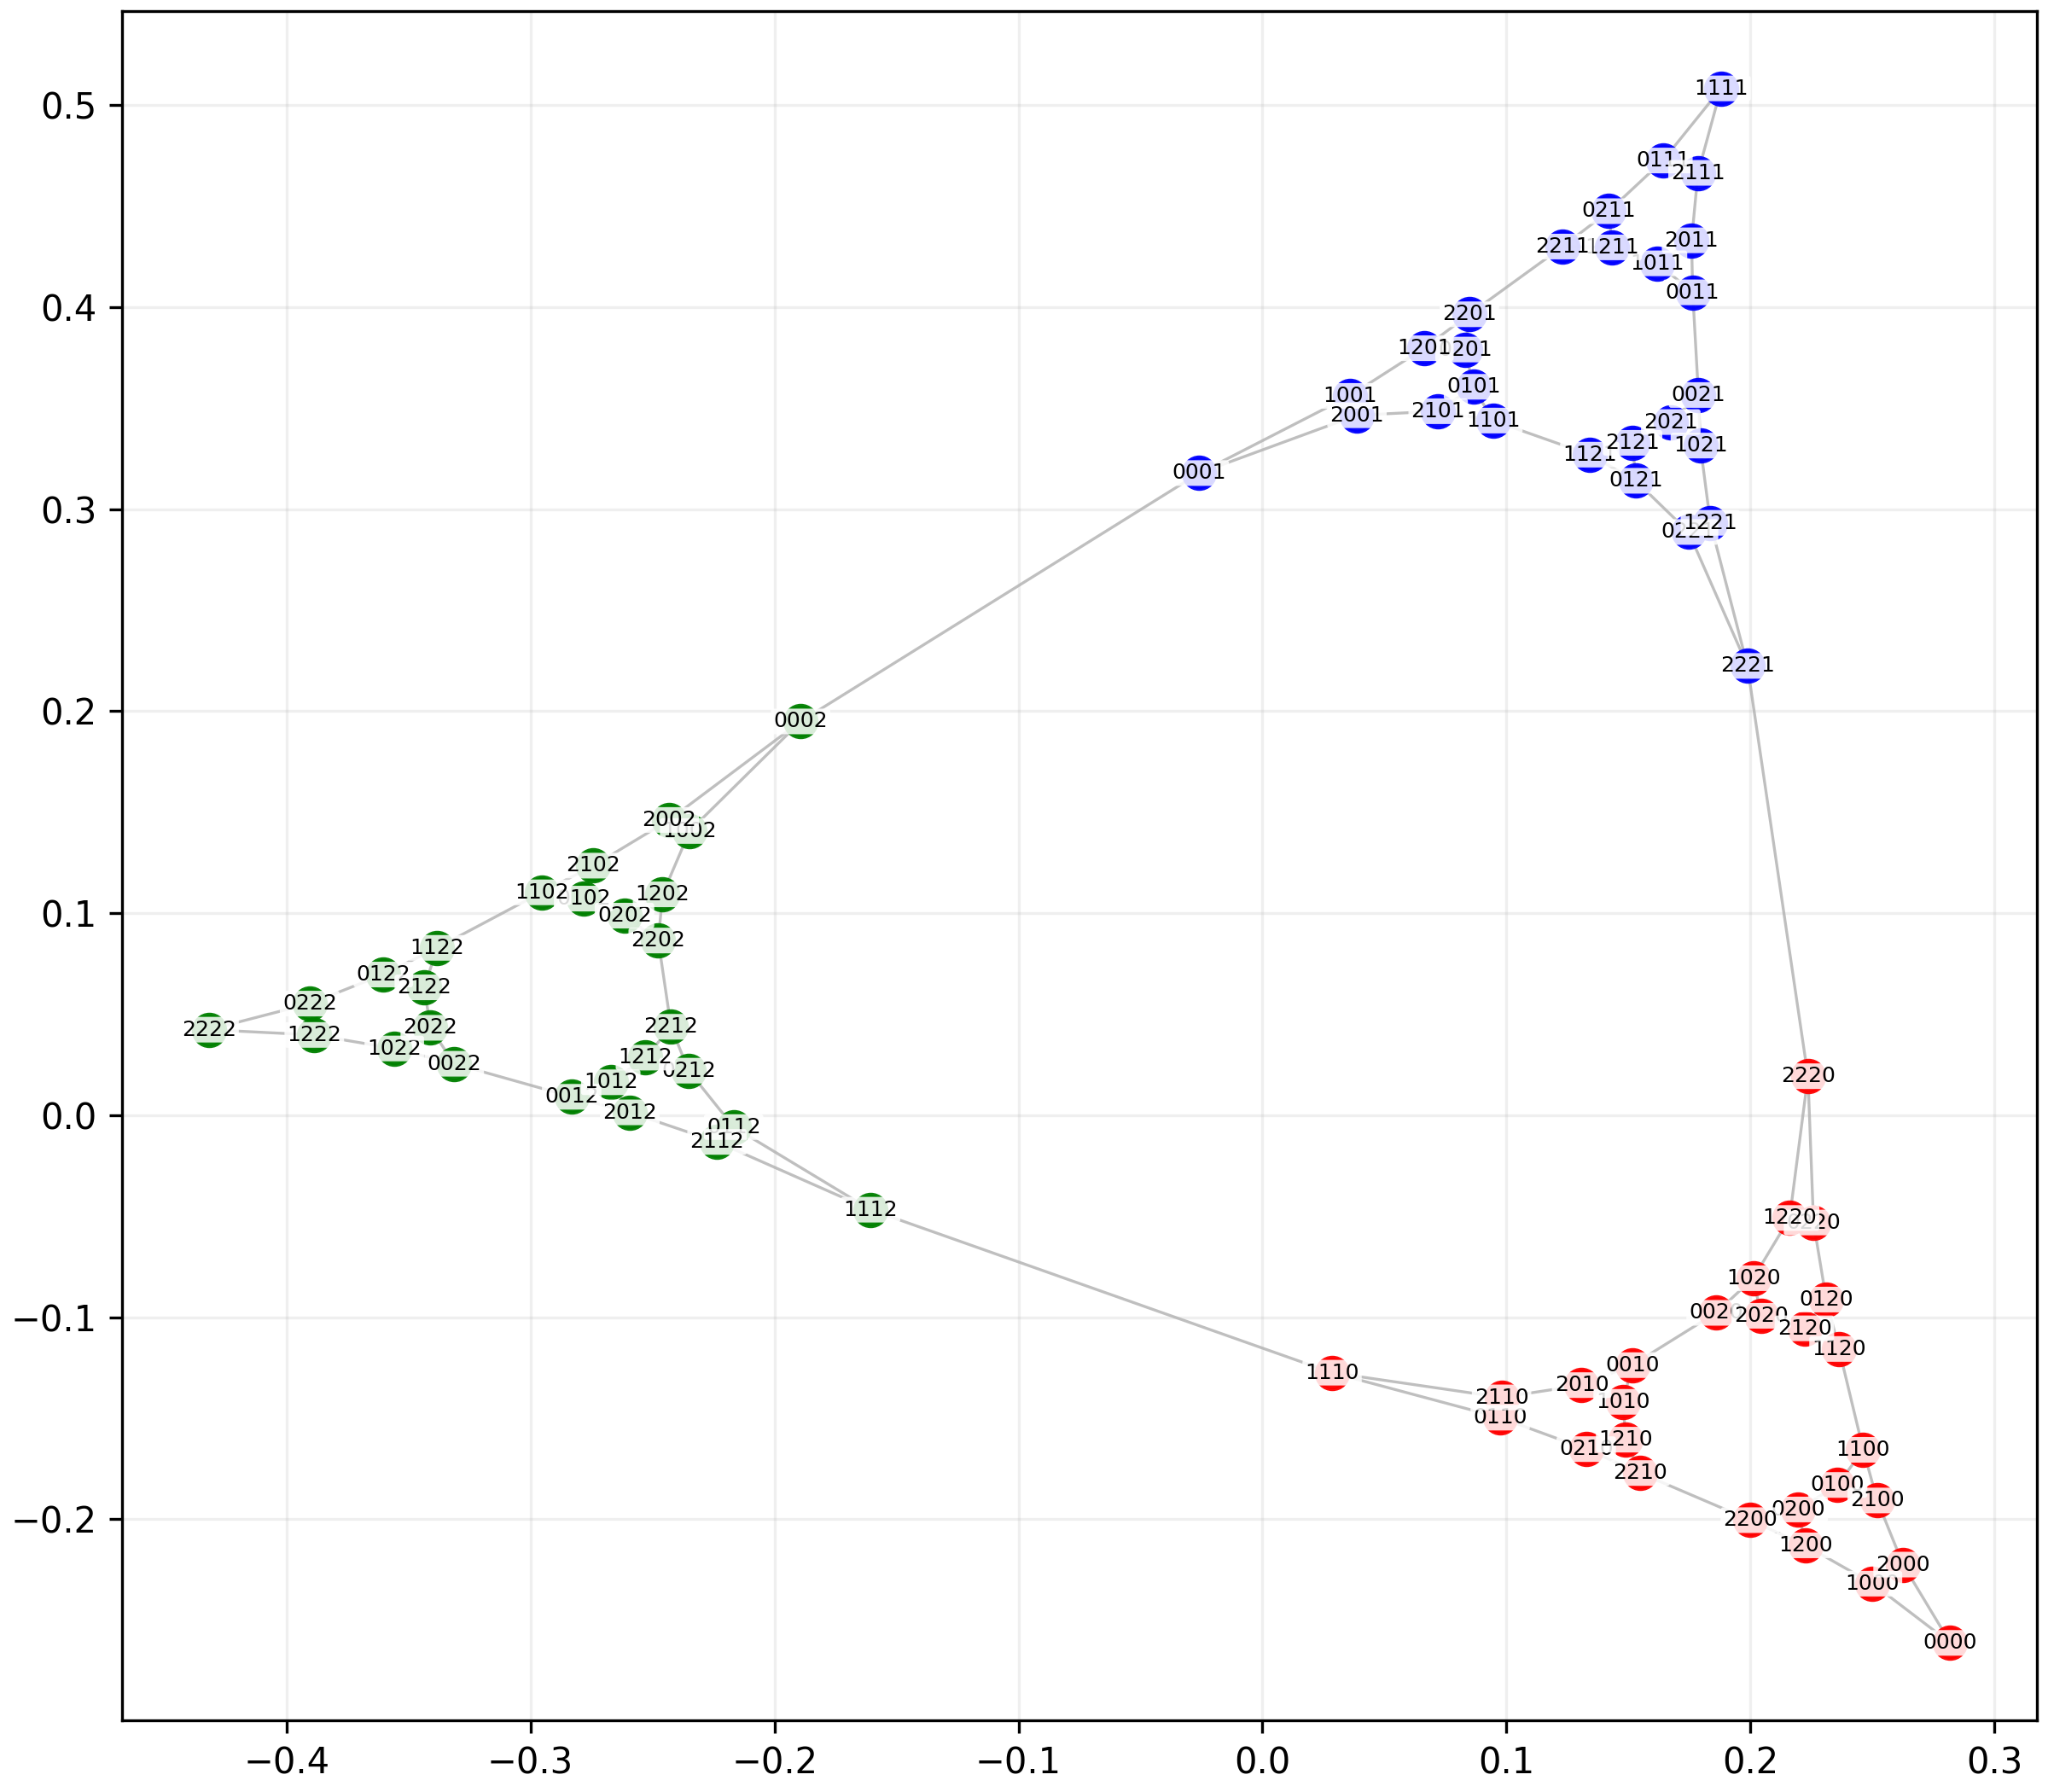
\includegraphics[width=\linewidth]{media/images/sae_sep_sae.png}\end{minipage}

\vspace{6pt}
\begin{minipage}{0.48\linewidth}\centering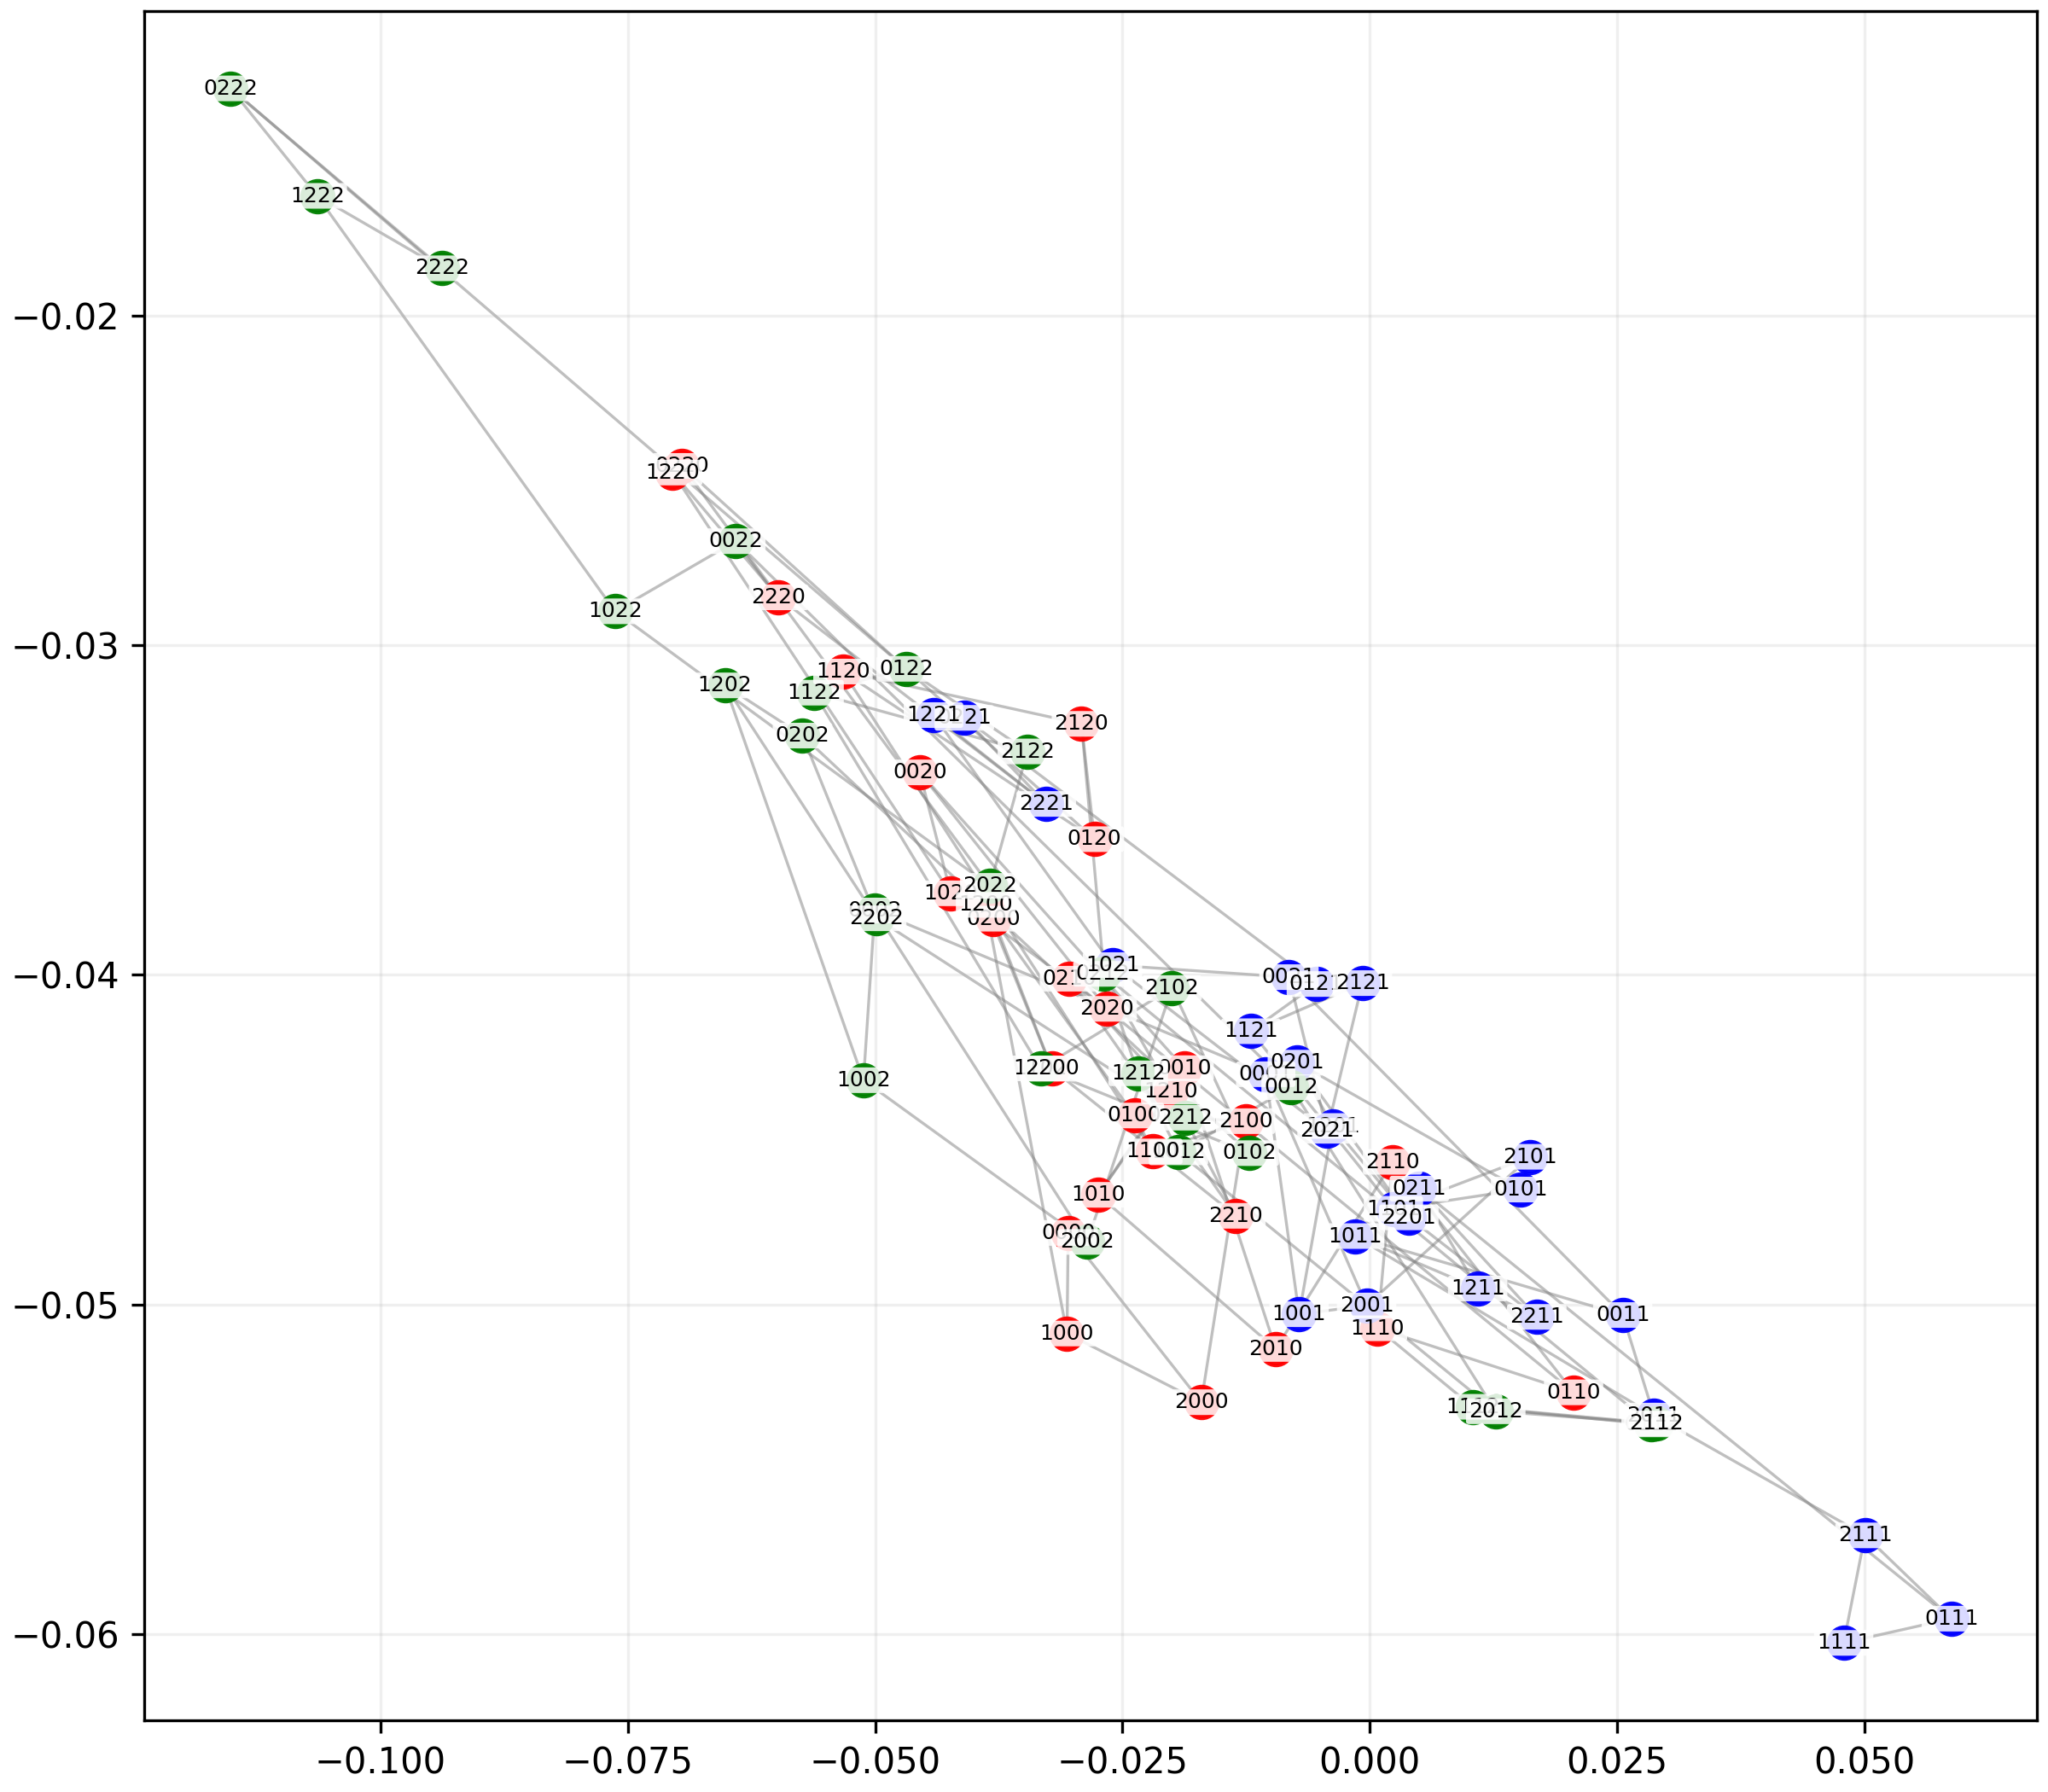
\includegraphics[width=\linewidth]{media/images/sae_move_raw.png}\end{minipage}\hfill
\begin{minipage}{0.48\linewidth}\centering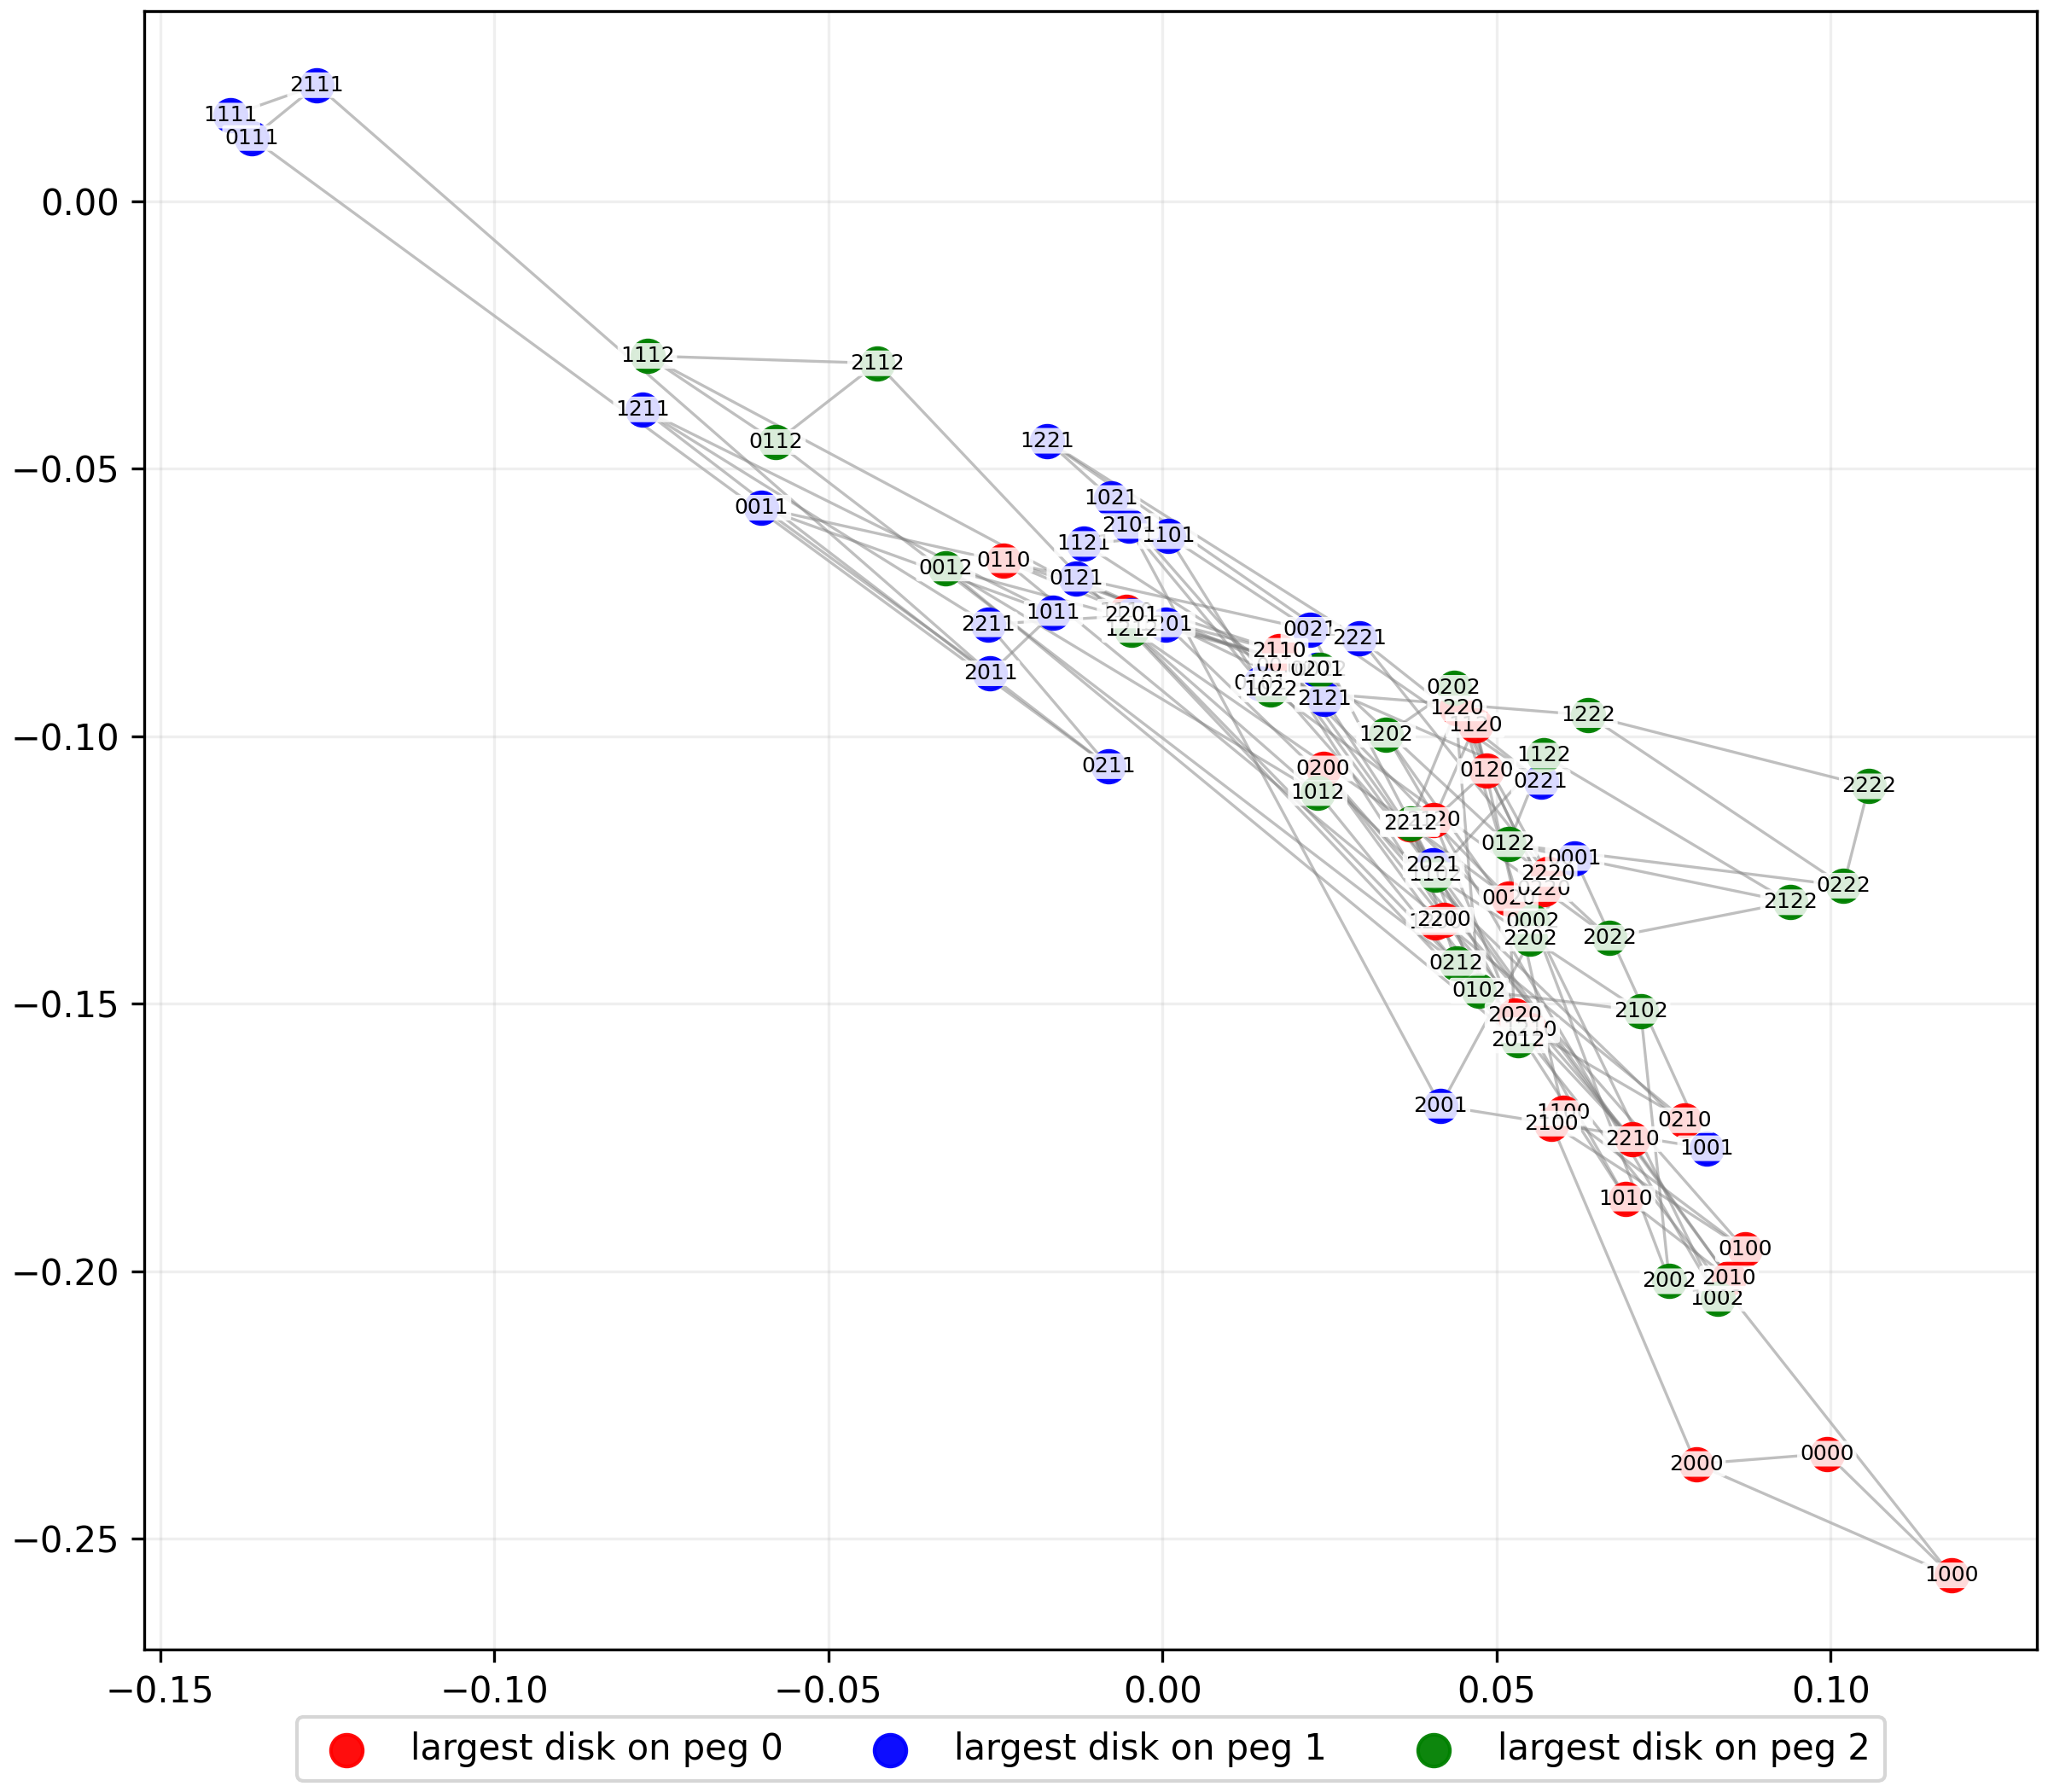
\includegraphics[width=\linewidth]{media/images/sae_move_sae.png}\end{minipage}
\end{minipage}
\caption{Distance-matching probe layouts at layer 5: raw residual stream (left) vs.\ SAE latents (right); SEP (top, raw $\rho{=}0.935$/SAE $\rho{=}0.935$) and move tokens (bottom, raw $\rho{=}0.136$/SAE $\rho{=}0.140$).}
\label{fig:sae}
\end{figure}

\section{Generation settings}
\label{app:gen}
Reasoning traces are generated with nucleus sampling ($T{=}1.0$, top-$p$ $0.95$, top-$k$ $20$).

\section{Tower-to-tower baselines}
\label{app:towertower}
On the standard tower-to-tower task all frontier reasoning models solve near-perfectly across $n\in\{3,4,5\}$ (DeepSeek-R1 24/25, Kimi-K2-Think 23/25, gpt-oss-120b 25/25, Qwen3.6-27B 24/25), confirming the task is saturated; the distilled DeepSeek-R1-Distill-Qwen-32B is the exception at 1/25.

\section{Full Position A probing}
\label{app:posA-full}
\begin{table}[h]
\centering
\caption{Position A (final prompt token) probing, three best and three worst layers by Spearman. Both models recover the configuration near-perfectly from middle depth. DS-32B denotes DeepSeek-R1-Distill-Qwen-32B.}
\label{tab:posA}
\begin{tabular}{llrrr}
\toprule
\textbf{Model} & \textbf{Layer} & \textbf{Spearman} & \textbf{Pearson} & \textbf{NS acc.} \\
\midrule
\multirow{6}{*}{Qwen3.6-27B} & 36 & \textbf{0.935} & \textbf{0.903} & \textbf{1.000} \\
 & 32 & \textbf{0.935} & \textbf{0.903} & \textbf{1.000} \\
 & 28 & \textbf{0.935} & \textbf{0.903} & \textbf{1.000} \\
 & 8  & 0.897 & 0.887 & \textbf{1.000} \\
 & 4  & 0.740 & 0.703 & 0.383 \\
 & 1  & 0.714 & 0.666 & 0.235 \\
\midrule
\multirow{6}{*}{DS-32B} & 8  & \textbf{0.936} & 0.906 & 0.975 \\
 & 44 & \textbf{0.936} & \textbf{0.908} & 0.988 \\
 & 32 & \textbf{0.936} & 0.906 & \textbf{1.000} \\
 & 60 & 0.917 & 0.907 & 0.790 \\
 & 64 & 0.862 & 0.833 & 0.642 \\
 & 1  & 0.730 & 0.704 & 0.580 \\
\bottomrule
\end{tabular}
\end{table}

\section{DeepSeek positions B and C}
\label{app:posBC-deepseek}
\begin{table}[h]
\centering
\caption{Probing DeepSeek-R1-Distill-Qwen-32B through generation (layers 24/36/48); columns as in \Cref{tab:posBC}.}
\label{tab:posBC-deepseek}
\begin{tabular}{llrrrrrr}
\toprule
\textbf{Position} & \textbf{Layer} & \textbf{Spearman} & \textbf{Acc} & \textbf{D0} & \textbf{D1} & \textbf{D2} & \textbf{D3} \\
\midrule
A & 24 & \textbf{0.935} & \textbf{1.00} & 0.68 & 0.56 & 0.68 & \textbf{0.89} \\
A & 36 & \textbf{0.935} & \textbf{1.00} & 0.61 & 0.61 & \textbf{0.73} & 0.86 \\
A & 48 & 0.933 & 0.98 & 0.62 & \textbf{0.63} & 0.63 & 0.83 \\
\midrule
B & 24 & 0.775 & 0.51 & 0.26 & 0.25 & 0.30 & 0.41 \\
B & 36 & 0.807 & 0.38 & 0.30 & 0.30 & 0.37 & 0.44 \\
B & 48 & 0.737 & 0.33 & 0.34 & 0.36 & 0.34 & 0.47 \\
\midrule
C & 24 & 0.894 & 0.71 & \textbf{0.77} & 0.46 & 0.50 & 0.51 \\
C & 36 & 0.899 & 0.68 & 0.64 & 0.48 & 0.52 & 0.51 \\
C & 48 & 0.863 & 0.57 & 0.50 & 0.41 & 0.50 & 0.51 \\
\bottomrule
\end{tabular}
\end{table}

\section{The four-disk Tower of Hanoi state space}
\label{app:sierpinski}
The state space of the four-disk Tower of Hanoi forms a Sierpi\'nski triangle (\Cref{fig:hanoi-4disk-state}): each node is a valid configuration and each edge a legal single-disk move. The three top-level sub-triangles partition the space by the position of the largest disk, the recursive cluster structure whose inflated cross-cluster separation produces the Spearman--Pearson gap reported throughout.

\begin{figure}[t]
    \centering
    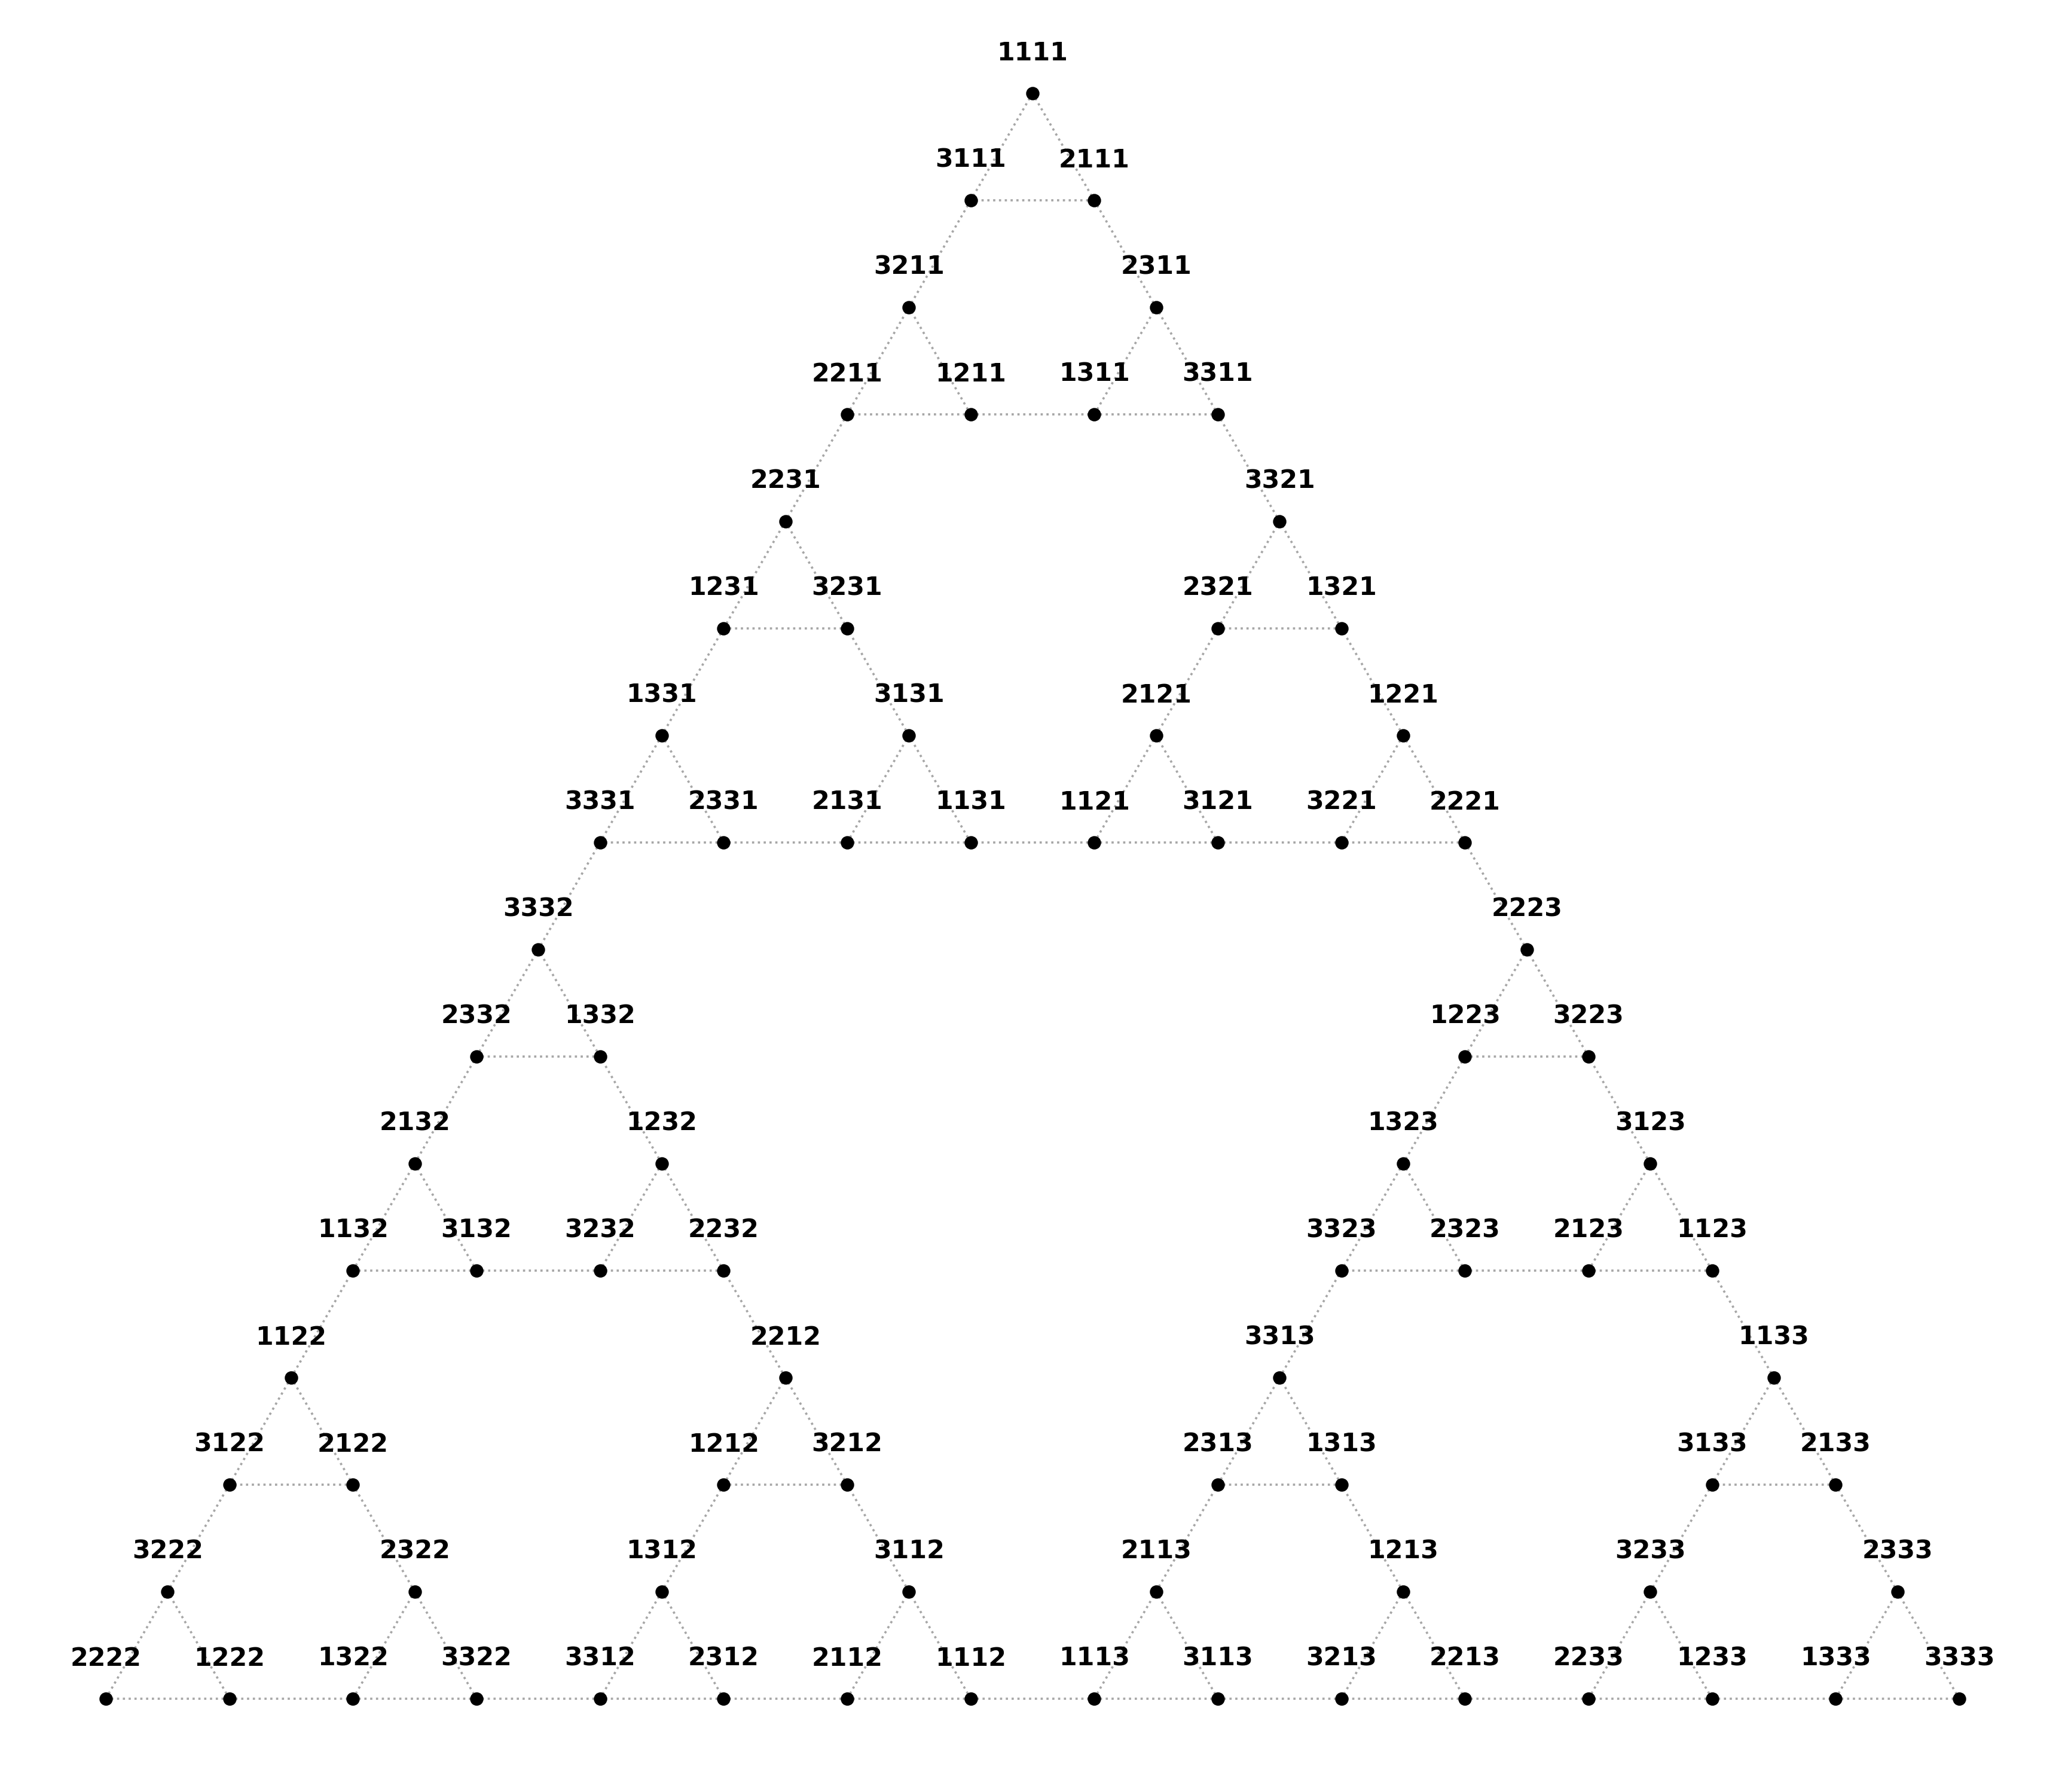
\includegraphics[width=0.8\textwidth]{media/images/sierpinski_4disk.png}
    \caption{The state space of the 4-disk Tower of Hanoi forms a Sierpi\'nski triangle. Each node is labelled by a triple indicating the peg on which each disk rests, ordered from smallest to largest. The three sub-triangles partition the space according to the position of the largest disk.}
    \label{fig:hanoi-4disk-state}
\end{figure}

\end{document}
